\documentclass[a4paper, 11pt]{article}
\usepackage{comment} % enables the us`e of multi-line comments (\ifx \fi) 
\usepackage{lipsum} %This package just generates Lorem Ipsum filler text. 
\usepackage{fullpage} % changes the margin
\usepackage{amsfonts}
\usepackage{amsmath}
\usepackage{amssymb}
\usepackage{graphicx}
\usepackage{amsthm}
\usepackage{svg}
\usepackage{enumitem}
\usepackage{color}
\usepackage{float}
\usepackage[utf8]{inputenc}
\usepackage{wrapfig}
\usepackage[arrow]{xy}
\usepackage{tikz-cd}


%%%%% Alphabets %%%%% 
\def\cA{\mathcal{A}}\def\cB{\mathcal{B}}\def\cC{\mathcal{C}}\def\cD{\mathcal{D}}\def\cE{\mathcal{E}}\def\cF{\mathcal{F}}\def\cG{\mathcal{G}}\def\cH{\mathcal{H}}\def\cI{\mathcal{I}}\def\cJ{\mathcal{J}}\def\cK{\mathcal{K}}\def\cL{\mathcal{L}}\def\cM{\mathcal{M}}\def\cN{\mathcal{N}}\def\cO{\mathcal{O}}\def\cP{\mathcal{P}}\def\cQ{\mathcal{Q}}\def\cR{\mathcal{R}}\def\cS{\mathcal{S}}\def\cT{\mathcal{T}}\def\cU{\mathcal{U}}\def\cV{\mathcal{V}}\def\cW{\mathcal{W}}\def\cX{\mathcal{X}}\def\cY{\mathcal{Y}}\def\cZ{\mathcal{Z}}

\def\AA{\mathbb{A}} \def\BB{\mathbb{B}} \def\CC{\mathbb{C}} \def\DD{\mathbb{D}} \def\EE{\mathbb{E}} \def\FF{\mathbb{F}} \def\GG{\mathbb{G}} \def\HH{\mathbb{H}} \def\II{\mathbb{I}} \def\JJ{\mathbb{J}} \def\KK{\mathbb{K}} \def\LL{\mathbb{L}} \def\MM{\mathbb{M}} \def\NN{\mathbb{N}} \def\OO{\mathbb{O}} \def\PP{\mathbb{P}} \def\QQ{\mathbb{Q}} \def\RR{\mathbb{R}} \def\SS{\mathbb{S}} \def\TT{\mathbb{T}} \def\UU{\mathbb{U}} \def\VV{\mathbb{V}} \def\WW{\mathbb{W}} \def\XX{\mathbb{X}} \def\YY{\mathbb{Y}} \def\ZZ{\mathbb{Z}}  

\def\bU{\mathbf{U}} \def\btU{\tilde{\bU}} \def\bUs{\bU^\circ}
\def\btUos{\btU_0^\circ}
\def\bG{\mathbf{G}} \def\bGs{\mathbf{G}^\circ}
\def\hol{\mathbf{hol}}
\def\bM{\mathbf{M}}
\def\bMs{\mathbf{M}^\circ}
\def\btUs{\btU^\circ} 
\def\xtild{\tilde{x}_0}
\def\utild{\tilde{u}_0}
\def\mtild{\tilde{m}_0}
\def\gamtild{\tilde{\gamma}}
\def\phitild{\tilde{\Phi}}
\def\tildphi{\tilde{\phi}}

\def\fa{\mathfrak{a}} \def\fb{\mathfrak{b}} \def\fc{\mathfrak{c}} \def\fd{\mathfrak{d}} \def\fe{\mathfrak{e}} \def\ff{\mathfrak{f}} \def\fg{\mathfrak{g}} \def\fh{\mathfrak{h}} \def\fj{\mathfrak{j}} \def\fk{\mathfrak{k}} \def\fl{\mathfrak{l}} \def\fm{\mathfrak{m}} \def\fn{\mathfrak{n}} \def\fo{\mathfrak{o}} \def\fp{\mathfrak{p}} \def\fq{\mathfrak{q}} \def\fr{\mathfrak{r}} \def\fs{\mathfrak{s}} \def\ft{\mathfrak{t}} \def\fu{\mathfrak{u}} \def\fv{\mathfrak{v}} \def\fw{\mathfrak{w}} \def\fx{\mathfrak{x}} \def\fy{\mathfrak{y}} \def\fz{\mathfrak{z}}
\def\fgl{\mathfrak{gl}}  \def\fsl{\mathfrak{sl}}  \def\fso{\mathfrak{so}}  \def\fsp{\mathfrak{sp}}  
\def\GL{\mathrm{GL}} \def\SL{\mathrm{SL}}  \def\SP{\mathrm{SL}}
\def\SO{\mathrm{SO}}

\def\<{\langle} \def\>{\rangle}
\def\ad{\mathrm{ad}} 
\def\Aut{\mathrm{Aut}}
\def\dim{\mathrm{dim}} 
\def\End{\mathrm{End}} 
\def\ev{\mathrm{ev}} 
\def\half{\hbox{$\frac12$}}
\def\Hom{\mathrm{Hom}} 
\def\qtr{\mathrm{qtr}} 
\def\tr{\mathrm{tr}} 
\def\Tr{\mathrm{Tr}} 
\def\vep{\varepsilon}

\def\ZZn{\ZZ/n\ZZ}
\def\acts{\rotatebox[origin=c]{-90}{$\circlearrowright$}}
%%%%%%%%%%%%%%%%%%%%%%%%%%%%%% 
%%%%%%%%%%%%%%%%%%%%%%%%%%%%%%


\begin{document}
\newtheorem{thm}{Theorem}[]
\newtheorem{Def}{Definition}[]
\newtheorem*{thm*}{Theorem}
\newtheorem*{def*}{Definition}
\newtheorem{lem}{Lemma}
\newtheorem*{rem}{Remark}
\newcommand{\shiftleft}[2]{\makebox[0pt][r]{\makebox[#1][l]{#2}}}
\newtheorem*{conj}{Conjecture}
\newtheorem{cor}{Corollary}[]

\newcommand{\compav}[1]{\textbf{\textcolor{blue}{#1}}}
\newcommand{\compat}[1]{\textbf{\textcolor{red}{#1}}}
\graphicspath{{images/}}
\setsvg{svgpath={./images/}}

% Title Page

\setlength{\topmargin}{1in} %top/bot margins
\setlength{\oddsidemargin}{\topmargin} %sidemargins

\setlength{\textheight}{11in} \setlength{\textwidth}{8.5in}
\setlength{\hoffset}{-1in} \setlength{\voffset}{-1in} \setlength{\evensidemargin}{\oddsidemargin} \addtolength{\textheight}{-2 \topmargin}\addtolength{\textwidth}{-2\oddsidemargin}
\setlength{\headheight}{0pt} \setlength{\headsep}{20pt} \setlength{\footskip}{20pt}
\addtolength{\textheight}{-\footskip} \addtolength{\textheight}{-\headheight} \addtolength{\textheight}{-\headsep}


\title{Periodic Geodesics on the Infinite Necker Cube Surface}
\author{Pavel Javornik}

\maketitle

%\begin{center}
%
%\includesvg[width=4.8in]{cubecoverphoto}\\
%\end{center}

\begin{abstract}
\noindent We classify all of the periodic and drift-periodic trajectories on the surface periodically constructed out of unit cubes lying on a plane in $\RR^3$. The Necker cube surface is a piecewise smooth Euclidean cone surface with neighborhoods locally isometric to the plane that gives up a natural piecewise isometry, or \emph{flattening}, onto a subset of $\CC$ with $\ZZ^2$ translational symmetries. We use the surface's topological properties to draw a connection between translation covers and rotational holonomy of closed curves by inducing fundamental group actions on the discrete space of attainable vectors via parallel transport along lifted paths. We then use the symmetries of this surface and its (branched) translation cover to show a correspondence between the space of attainable (rational) geodesics of the Necker cube surface, their dynamical properties, and the translation cover's \emph{Veech group}. The ``slope" of a geodesic is represented by a relatively prime pair of integers, which is used to tell not only whether or not a geodesic with this initial direction (relative to choice of basis in its initial tangent space) closes, but the overall length of the trajectory as a function of its components.
\end{abstract}
\begin{figure}[H]
\centering
\includesvg[width=4in]{cubesxyzpaths2bwv2b}
\label{fig:front}
\caption{Periodic and drift-periodic geodesics on the Necker cube surface}
\end{figure}
\newpage
\section{Introduction}
The Necker cube has been studied extensively due to its interesting effects on human visual perception. \cite{Albert} A popular adaptation of the Necker cube is the edge-to-edge pairing of multiple solid cubes giving the illusion of a rhombile tiling of the plane when viewed from a fixed angle. (Fig 1) It is most recognizable in the works of M.C. Escher \cite{Escher1}\cite{Escher2} and as the game board in the 80s cabinet arcade classic, $\text{Q}^*\text{bert}$.\cite{Qbert} The cube was named after the Swiss crystallographer Louis A. Necker for having been one of the first people to study the wire-frame cube's properties as an optical illusion. 

 The solid presentation of the cube, rendered as a flat surface with three rear faces obscured from view, achieves a similar effect to the ``wire-frame" version when infinitely many are arranged along their outer edges. The semi-cube is a construction obtained by removing these obscured faces and making translational identifications on these edges that is homeomorphic to the two-dimensional torus. The Necker cube surface is itself obtained by gluing infinitely many copies of the semi-cube surface along those outer edges. (Fig ??)


An infinite surface like the Necker cube is piecewise smooth and \emph{flat} on its smooth sections. Neighborhoods contained in these faces are isometric to the Euclidean plane. The tangent space at a point is the vector field contained in a plane tangent to the surface. A vector field translated along a closed loop on this surface induces a phenomena known as \emph{rotational holonomy}. This is a linear transformation (element of $\SO(2,\RR)$ for orientable manifolds) between tangent spaces at the initial and terminal point of the loop. When a surface is flat, deformations of the loop do not alter its holonomy. Furthermore, a contractible (trivial) loop has trivial holonomy due to the local plane isometry on its smooth sections. In this case any homotopic path will induce the same linear transformations, and that gives up a well-defined group action on the tangent bundle of the surface by the first fundamental group of the surface.

In studying geodesics on an infinite flat surface, it is important to make this connection early on. The rotational holonomy group acts transitively on the holonomy bundle, a principal bundle of tangent spaces over a point on the surface. This holonomy group is used to construct a covering space where the only closed loops are those with trivial holonomy. In desirable cases, the holonomy group is discrete and this cover has finitely many sheets. This surface is known as an infinite \emph{translation surface}. It is on this surface that geodesics behave as they would when projected back down to the flat surface. In the context of Riemann surfaces, a translation surface is a surface with a maximal translational atlas, i.e. every transition function on images of neighborhoods in $\CC$ is an affine translation. The surface inherits a flat metric from pulling back the Euclidean metric on $\CC$. On such a surface the principal holonomy bundle of tangent spaces over a point consists of a single vector space. Combining these two facts, in local coordinates any geodesic in direction $\theta\in\RR/2\pi\ZZ$ on this surface is isometric to $te^{i\theta}$ for $t\in\RR$. [cite Zorich]
\begin{rem}
Familiarity is assumed on the part of the reader with covering space theory, translation (particularly Veech) surfaces, and their associated Veech groups. For general surveys on these topics we refer readers to: [cite], [cite].
\end{rem}

\subsection{Directions and Trajectories}
What originally motivated this research was the appearance and symmetries of computer simulated geodesics on the surface. These symmetries are related to the reflective and rotational symmetries of its translation cover.
\begin{figure}[H]
\centering
\includesvg[width=4in]{oddoddtrajectory}
\caption{A closed trajectory on the Necker cube surface modeled using sage-flatsurf \cite{flatsurf} and various sage utilities. [cite]}
\end{figure}
We began finding patterns between the choice of initial direction and periodicity. What we aimed to find out was what geometric properties of the surface relate a geodesic's dynamical characteristics to its initial trajectory angle. The answer to the question of what directions determine periodicity and drift periodicity turned out remarkably simple. Along the way we learned that the symmetries of this surface and its various covers gave up not only a clear distinction between periodic and drift-periodic trajectories, but the total arclengths of these paths after a single period. For example the previous figure's geodesic has an initial trajectory angle $\tan^{-1}(51/31)\approx58.71^\circ$, and total total length of $6\sqrt{3562}\approx 358.09$. Appendix [include appendix] showcases various geodesics, their initial trajectory angles, and total lengths. 

\subsection{Discussion of Results}
A surface composed of infinitely many cubes is endowed with a flat metric and local plane isometries. Via the parallel transport of a unit vector tangent to the surface along a geodesic, we view its image as a sequence of straight lines on the smooth faces of the surface. (Fig 2) A geodesic is no doubt a piecewise curve in space. Let $\bUs$ be the connected, topological space known as the Necker cube surface.
\\\newpage
\begin{wrapfigure}{l}{1.9in}
\includesvg[width=1.7in]{vectorplane}
\end{wrapfigure}
\noindent Let $u_0$ be a point on the surface that is contained in the interior of a face and consider a tangent unit vector $v\in T_{u_0}(\bUs)$, the tangent vector field over $u_0$. A flattening map acts as an atlas on the smooth sections of $\bUs$ (see section [find section]) is an affine map from the surface to $\RR^2$ with a derivative in $\SO(3,\RR)$ that   (See section [?] in Appendix [Include section or appendix on this map].)
\\\\
Let the angle $v_0$ makes relative to a choice of basis (orthogonal vectors parallel to $\bUs$'s faces) be the \emph{initial trajectory angle} of a \emph{unit-speed geodesic} based at $u_0$, $\Phi_t:\RR\rightarrow\bUs$. The initial trajectory angle is said to be $\emph{rational}$ if there is some $k\in\RR$ such that $kv_0$'s nonzero components are relatively prime integers. A rational initial trajectory angle in $\RR^2$ falls into one of two categories:
\begin{Def}
Let $v_0$ be a rational unit vector of the form $\frac{1}{k}(x,y)\in\RR^2$ with $x,y\in\mathbb{Z}$ and $k=\sqrt{x^2+y^2}\in\mathbb{R}$. We say $kv_0$ is an \textbf{odd-odd} vector if $x,y$ are relatively prime and both odd. We denote the \textbf{set of all odd-odd directions} $\mathcal{O}$. We say that $kv_0$ is an \textbf{even-odd} vector if $x,y$ are relatively prime and of opposite parity. We denote the \textbf{set of all even-odd directions} $\mathcal{E}$. Finally, $\cS=\cO\sqcup\cE$ is the \textbf{collection of all possible rational directions}.
\end{Def}
\noindent It may be more helpful to think of an element in $\cS$ as the slope of $\Phi$, given $\bUs$'s flat structure. Recall that a geodesic on the surface is \emph{periodic} if there exists some $T>0$ such that $\Phi(t+T)=\Phi(t)$ for all $t\in\RR$, and \emph{drift-periodic} if there exists some $T'>0$ and non-trivial translation, $f$, such that $\Phi(t+T')=f(\Phi(t))$ for all $t\in\RR$. In any case we call this value the \emph{period} of $\Phi$ if it is the \emph{smallest} possible value that satisfies this. We additionally require that at no point does $\Phi$ encounter a cone singularity of the surface, where geodesic behavior is undefined. We call these well behaved geodesics \emph{non-singular}. We use $||~||:\RR^2\rightarrow\RR_{\geq 0}$ to denote the standard Euclidean norm in $\RR^2$.

\begin{thm*} \textbf{Periodic and Drift-Periodic Geodesics on the Necker cube surface.} 
\\Let $\Phi_t:\RR\rightarrow\bUs$ be a non-singular unit-speed geodesic on the Necker cube surface such that $\Phi(0)=u_0$ and $\Phi'(0)=v\in\RR^3$. Let $v_0\in\RR^2$ be a distance-preserving projection of $v$ onto the plane tangent to the surface at $u_0$. Let $k\in\RR$ such that $kv_0\in\cS$. Then the following is true:
\begin{enumerate}[label=(\roman*)]
\item $\Phi$ is periodic if $kv_0\in\cO$ with period $T=6||kv_0||$.
\item $\Phi$ is drift-periodic if $v_0\in\cE$ with period $T=2||kv_0||$.
\end{enumerate}
\end{thm*}

There is a very clear dynamical dichotomy at work when it comes to $\Phi$'s slope, not unlike the well-known Ehrenfest Wind-Tree model with $\frac{1}{2}\times\frac{1}{2}$ square obstacles distributed on a $\ZZ^2$ lattice. [cite]

\subsection{Acknowledgements}
-Pat Hooper\\
- Vincent Delecroix, Ferrán Valdez, pascal hubert\\
- \\

\newpage

\section{Periodic Construction of the Surface}
This section will detail how the Necker Cube surface is constructed as a covering space of a thrice-punctured torus. We begin by making the following identifications on 3 unit squares:
\begin{figure}[H]
\centering
\includesvg[width=1.83in]{neckercube}\includesvg[width=2in.]{neckercubepath}
\caption{$\bGs$ with and without paths $a,b,c,d$.}
\end{figure}

We will call this ``half-cube" $\bG$. It is a piecewise smooth surface homeomorphic to the torus. Every vertex is a cone singularity of the surface with cone angle $3\pi$ or $\frac{3\pi}{2}$. Let $\Sigma_{\bG}\subset\bG$ be the set of these singularities. We use $\bG\backslash\Sigma_{\bG} = \bGs$ to denote the surface punctured at these points. The paths labeled $a,b,c,d$ are independent of one another and generate $\bGs$'s fundamental group, $\pi_1(\bGs)\cong \<a,b,c,d \>$, the free group of four generators. (Figure ?) The unpunctured Necker cube surface $\bU$ is embedded in $\RR^3$ by gluing along $\bG$'s outer edges (marked with solid triangles):

\begin{figure}[H]
\centering
\includesvg[width=4in]{neckercubepathsurface}
\end{figure}
From this diagram we see that $\bU$ is a universal cover of $\bG$. In this paper we are studying geodesic behavior on $\bU$ and, in order to do so properly, it is necessary to determine how the parallel transport of a unit vector around a cone singularity acts on the unit tangent bundle of the surface. But to study a given path's rotational holonomy, we require that these loops (see $c,d$ in Fig 3) aren't contractible through the cube's sharp corners. To that effect, we puncture the surface at these points.  Denote the countably infinite set of singularities of $\bU$ by $\Sigma_{\bU}$. The \emph{Necker cube surface} is the punctured surface $\bUs=\bU\backslash\Sigma_{\bU}$. Observe from the previous diagram that $\pi_1(\bUs)$ is the kernel of the following group homomorphism on $\pi_1(\bGs)$:

\begin{Def}
Let $\varphi_1:\pi_1(\bGs)\rightarrow \ZZ^2$ be the homomorphism on a free group given by $c,d\mapsto(0,0)$, $a\mapsto(1,0)$, and $b\mapsto(0,1)$.
\end{Def}

The cover of $\bGs$ with fundamental group $\ker\varphi_1$ is the space $\bUs=\tilde{\mathbf{G}}^\circ/\ker\varphi_1$ where $\ker\varphi_1$ acts on $\bGs$'s universal cover $\tilde{\mathbf{G}}^\circ$ by deck transformations.

\begin{Def}
Let $p_1:\bUs\rightarrow\bGs$ be a projection that induces a monomorphism on the fundamental groups of these surfaces such that $p_{1*}\pi_1(\bUs)=\ker\varphi_1$.
\end{Def}

It follows that $(\bUs,p_1)$ is a covering space of $\bGs$. We say $\Delta_{p_1}=\pi_1(\bGs)/p_{1*}\pi_1(\bUs)\cong\ZZ^2$ is the \emph{deck group} of the covering isomorphic to the group of deck transformations of $p_1$ $-~\text{Deck}_{p1}(\bUs)$. Using the fact that this cover is regular, we say that $p_1(\bUs)=\bUs/\ZZ^2$ and $\bGs$ is a quotient of the Necker cube surface. Apply the following cutting and gluing operations to $\bGs$: \\
\begin{figure}[H]
\centering
\includesvg[width=3in]{LTorus}
\end{figure}
\noindent This L-shaped torus is then taken apart and recovered as $2\times 2$ torus missing a unit square with the following edges identified:\\
\begin{figure}[H]
\centering
\includesvg[width=2in]{BranchTorus}
\caption{$\bGs$ and its paths after reconstruction.}
\end{figure}

Consider a $2\times2$ sheet missing an open unit square and that square's vertices (punctures). Center this structure around $0\in\CC$ and recover $\bGs$ with the identifications made in Fig ??. Let $m,n\in\ZZ$. Similar identifications can be made on the following subset of $\CC$ to recover $\bUs$:

\begin{equation}
\label{eq:P}
\mathbf{P} = \mathbb{C}\text{ }\backslash\bigcup_{m,n \in {\mathbb Z}} \big{\{} u+vi:~|u-2m|<\frac{1}{2},~|v-2n|<\frac{1}{2},~u=2m\pm\frac{1}{2}~v=2n\pm\frac{1}{2} \big{\}}.
\end{equation}

\begin{figure}[H]
\centering
\includegraphics[width=2.8in]{P.png}
\end{figure}
\compav{shade the surface}
\noindent Let $m,n\in\ZZ$. The coordinate $c_{m,n}=(2m+i2n)\in\CC$ is the center of a removed square. The set of all centers form a lattice in the plane that uniquely identifies every section in the fiber over $\bGs$ under $p_1$ with an element of $2\ZZ[i]$. Now let $\zeta_{m,n}(t)=(2m+t)+i(2n-\frac{1}{2})$ and 
$\xi_{m,n}(t)=(2m+t)+i(2n+\frac{1}{2})$ be paths on $\mathbf{P}$ that run along the top and bottom edges of the squares, parameterized by $t\in (-\frac{1}{2},\frac{1}{2})$ and $(m,n)\in\ZZ^2$. These paths are oriented so that edge identifications can be made by translations and rotations relative to $(m,n)$. (see figure above) $\bUs$ is recovered as the topological quotient $\mathbf{P}/\sim$, where $\sim$ is the following minimal relation on $\mathbf{P}$:

\begin{equation}
\begin{split}
\zeta_{m,n}(t)\sim i[\zeta_{m,n}(t)-c_{m,n}]+c_{m,n}-1\\
\xi_{m,n}(t)\sim i[\xi_{m,n}(t)-c_{m,n}]+c_{m,n}+1
\label{eq:rel2}
\end{split}
\end{equation}
The translations, $\pm 2,\pm 2i$, on $\mathbf{P}$ are isometries that preserve these identifications and induce isomorphisms of $\bUs$. We denote the isomorphism induced by $+2$ as $f_h$, for horizontal, and the isomorphism induced by $+2i$ as $f_v$, for vertical:

\begin{figure}[H]
\centering
\includesvg[width=2.3in]{tiling}
\end{figure}

From this image it's clear that the group generated by these horizontal and vertical isomorphisms under function composition, $\<f_h,f_v~\vert~[f_h,f_v] \>$, form $\text{Deck}_{p_1}(\bUs)$. Let $x_0\in\bGs$ and fix a point in the fiber, $u_0\in p_{1}^{-1}(x_0)\subset\bUs$. We consider the groups $\pi_1(\bUs,u_0)$ and $\pi_1(\bGs,x_0)$. There is a well-defined transitive action of the group $\pi_1(\bGs,x_0)$ on the set $p_{1}^{-1}(x_0)$ by lifting a loop on $\bGs$ to a curve on $\bUs$ based at a point in the fiber, and sending it to the terminal point of the lift. [cite that algebraic top book 5.7, beginning pg.133]. A curve is a continuous map from $[0,1]$ to the surface, and a loop is a closed curve where the terminal and initial point coincide.

\begin{thm}
Let $a,b\in\pi_1(\bGs,x_0)$ be the homotopy class generators as in Figure [??]. Let $\tilde{a},\tilde{b}$ be $u_0$-based lifts of a loop in $a,b$ onto $\bUs$. Then $\tilde{a}(1)=f_h(u_0)$ and $\tilde{b}(1)=f_v(u_0)$.
\end{thm}

\begin{cor}
Let $\alpha\in\pi_1(\bGs,x_0)$. Denote the unique $u_0$-based lift of a loop in $\alpha$ to $\bUs$ as $\tilde{\alpha}$. If $\varphi_1(\alpha)=(m,n)$, then 
\begin{align}
\tilde{\alpha}(1)=(f_h^m\circ f_v^n)(u_0).
\end{align}
\end{cor}
This just follows from the previous theorem as $c,d$ are mapped trivially, and under $\varphi_1$ a word in $\pi_1(\bUs)$ is taken to commutative automorphisms of $\bUs$. For shorthand, we will use $f_\alpha$ to denote the \emph{induced deck transformation.} 

\begin{lem}
$f_\alpha$ is a local diffeomorphism of the surface $\bUs$. 
\begin{proof}
Consider a 
\end{proof}
\end{lem}

\subsection{Embedding the Necker cube surface}
In this section we define a map from $\bUs$'s $\RR^3$ embedded form to $\mathbf{P}$. The isomorphisms induced from translations on $\mathbf{P}$ are local diffeomorphisms on the smooth sections of $\bUs$, $S(\bUs)$, that relate the fundamental group of $\bGs$ to the tangent spaces of $p_1^{-1}(x_0)$. $S(\bUs)$ is the set of faces of cubes without boundary that are isometric to the plane. Let $m,n,l\in\ZZ$. A topologically equivalent notion of the (unpunctured) Necker cube surface is as the union of sets:  \\
\begin{align*}
\mathbf{A}=\bigcup\big{\{}\mathbf{A}_{m,n,l}: m+n+l=0\big{\}},
\\\mathbf{B}=\bigcup\big{\{}\mathbf{B}_{m,n,l}: m+n+l=0\big{\}},
\\\mathbf{C}=\bigcup\big{\{}\mathbf{C}_{m,n,l}: m+n+l=0\big{\}},
\end{align*}
which correspond to the following families of ``half-cubes" based integer points on a plane in $\RR^3$:

\vspace{0.2in}
\begin{tabular}{p{10cm}c}
\begin{align*}
\mathbf{A}_{m,n,l} = [m, m+1]\times[n,n+1]\times\{l\}, 
\\\mathbf{B}_{m,n,l} = \{m+1\}\times[n,n+1]\times[l-1,l],
\\\mathbf{C}_{m,n,l}= [m,m+1]\times\{n+1\}\times[l-1,l].
\end{align*}
&
\shiftleft{0.3in}{\raisebox{-1in}{
\includegraphics[scale=1]{label.png}}}
\end{tabular}

\begin{figure}[H]
\centering
\includesvg[width=1in]{cubesxyzcut}
\caption{Embedding the Necker cube surface, i.e. $\bU=\mathbf{A}\cup\mathbf{B}\cup\mathbf{C}$.}
\end{figure}


\compav{use different symbol for embedding maybe $\bUs_{\RR^3}$}\\
Of course $\bUs$ is just the exclusion of the semi-cube vertices. Then by removing the edges of each cube, we obtain $S(\bUs)$. Identify $\mathbf{P}\subset\CC$ with $\RR^2$ in the usual way, $(1,0)\sim 1$ and $(0,1)\sim i$. We say $\Psi:\RR^3\rightarrow\RR^2$ is a piecewise linear map from $\bUs$ to $\mathbf{P}$ given as
\begin{equation}
\Psi\left[\begin{array}{c}
	x\\y\\z
\end{array}\right] 
= 
\begin{cases}
	\left[ \hspace{2mm} \begin{matrix}
		1 & 0 & 0 \\
		0 & 1 & 0 \\
	\end{matrix}\hspace{3mm}\right]

	&\left[\begin{array}{c}
	x - m
	\\ y- n
	\\ z - l
	\end{array} \right]
	+
	\left[\begin{array}{c}
		2m - \frac{3}{2}
		\\ 2n - \frac{3}{2}
	\end{array} \right]
		\text{if } (x,y,z)\in \mathbf{A}_{m,n,l}	\vspace{2mm}
	\\
		
		
	\left[ \begin{matrix} \hspace{2mm}
	0 & 0 & -1 \\
	0 & 1 & 0 
	\end{matrix}\hspace{2mm}\right]
	&\left[\begin{array}{c}
		x - m
		\\ y- n
		\\ z - l
		\end{array} \right]
	+
		\left[\begin{array}{c}
			2m - \frac{1}{2}
			\\ 2n - \frac{3}{2}
		\end{array} \right]
		 \text{if } (x,y,z)\in \mathbf{B}_{m,n,l}	\vspace{2mm}
	\\
	
		\left[ \begin{matrix} \hspace{2mm}
		1 & 0 & 0 \\
		0 & 0 & -1 
		\end{matrix}\hspace{2mm}\right]
		&\left[\begin{array}{c}
			x - m
			\\ y- n
			\\ z - l
			\end{array} \right]
		+
			\left[\begin{array}{c}
				2m - \frac{3}{2}
				\\ 2n - \frac{1}{2}
			\end{array} \right]
				 \text{if } (x,y,z)\in \mathbf{C}_{m,n,l}	\vspace{2mm}
\end{cases}
\end{equation}

The inverse of this map would have to recover one of the coordinates as a function of the other two. To recover a section of $\Psi(\mathbf{A})$, for example, the z-coordinate would be $-(m+n)$. The rest are not difficult to determine. To see this particular setup used in modeling geodesics, we refer the reader to a flatsurf demonstration. [cite]

\begin{thm}
Let $\Psi=\{\Psi_{A_{m,n,l}},\Psi_{B_{m,n,l}},\Psi_{C_{m,n,l}}~:~m+n+l=0 \}$. Then $\Psi$ is a complex atlas on $\bUs_{\RR^3}$.
\begin{proof}
Clearly these charts cover the surface. Observe from the following diagram that there are finitely many intersections of any two neighborhoods that coincide with an edge on the cube centered at $(m,n,l)$. There are only 9 edges to consider since every cube is punctured at its vertices.
\begin{figure}[H]
\centering
\includesvg[width=4in]{edgegraph}
\end{figure}
A transition function on the four edges of the $\mathbf{A}$ face is obtained as the identity just by setting $x$ or $y$ to $m\pm1$ or $n\pm1$. Similarly, from $\mathbf{B}_{m,n,l}$, $\mathbf{C}_{m,n,l}$ to $\mathbf{A}_{m+1,n,l-1}$ and $\mathbf{A}_{m,n+1,l-1}$, these values coincide. The trickier ones to show are the transition functions on the 3 vertical edges. These are the edges that split when mapped onto $\mathbf{P}$. \\
Let $t\in(-\frac{1}{2},\frac{1}{2})$. Consider the following parameterization of these edges:
\begin{align*}
a(t):=&(m+1,n,l-\frac{1}{2}+t)\\
b(t):=&(m,n+1,l-\frac{1}{2}+t)\\
c(t):=&(m+1,n+1,l-\frac{1}{2}+t)\\
\end{align*}  

\compav{Show that the transition functions are given by the identification $\sim$ on $\mathbf{P}$.}

By induction on these integers, it naturally follows that this is true of the entire Necker cube surface.
\end{proof}

\end{thm}

Therefore this surface is Riemann. In addition, $(\bUs,\Psi)$ respects the edge identifications made on $\mathbf{P}$ and the two are topologically equivalent. 

\compav{come back to the discussion of holonomy}

Let $\gamma:[0,1]\rightarrow\bUs$ be a curve on the surface with $\gamma(0),\gamma(1)\in S(\bUs)$. If $\gamma(0)$ and $\gamma(1)$ are not contained in the same face, then $\gamma$ is a piecewise smooth curve.

Since this surface is obtained as a regular cover of $\bGs$, it has a complex structure and Riemannian connection, $\triangledown$, on the tangent bundle of the surface, $T\bUs=\bigcup_{p\in\bUs}T_{p}(\bUs)$. This implies the existence of parallel translation maps of vector fields along $\gamma$ and a linear isomorphism between tangent spaces $T_{\gamma(0)}(\bUs)$ and $T_{\gamma(1)}(\bUs)$. [cite Loring W. Tu Dif Geometry] The Necker cube surface is \emph{flat} and admits zero curvature throughout. Let $\gamma$ be a closed loop on $\bUs$ based at $u_0\in p_1^{-1}(x_0)$. If $u_0$ is contractible to a point, then it would act trivially on $T_{u_0}$. [Sharpe,1997] Let $v_0\in T\bUs_{\gamma(0)}$. Let $P_\gamma:T\bUs_{u_0}\rightarrow T\bUs_{u_0}$ be the parallel transport map given up by the connection $\triangledown$ along the loop $\gamma$. The \emph{rotational holonomy group} is the set of all parallel transport maps given up by closed loops $\gamma$, $\text{Hol}_{u_0}(\triangledown)$. This forms a subgroup of $\SO(2,\RR)$ that acts on $T_{u_0}(\bUs)$. [cite Santoro] 


\subsection{Rotational Monodromy Group}
A \emph{rotational monodromy map} is a homomorphism from the fundamental group of a surface to the \emph{rotational holonomy group} acting on the unit tangent space via parallel transport of a vector along a curve in its homotopy class. Existence of a parallel transport map is a consequence of an affine connection on a Riemann surface. On an oriented surface, the rotational holonomy group is an element of $\SO(2,\RR)$ that associates a loop with a linear isomorphism of the tangent space upon returning to the initial point. When the surface is \emph{flat}, contractible loops have trivial linear holonomy and will parallel transport a vector on a tangent vector field along any contractible loop without rotating it. [cite Zorich] In this case, rotational monodromy is well-defined and maps the fundamental group of a surface to a subgroup of $\SO(2,\RR)$.

\begin{Def}
Let $I_2=\begin{bmatrix}1 & 0\\0 & 1\end{bmatrix}$ and $R=\begin{bmatrix}0 & -1 \\1 & 0\end{bmatrix}$. \\
The map $\varphi_2:\pi_1(\bGs)\rightarrow SO(2,\ZZ)$ is the group homomorphism given by \\$a,b \mapsto I_2$ \\$c  \mapsto R$\\$d  \mapsto R^3$.
\end{Def}

\begin{figure}[H]
\centering
\includesvg[width=2.5in]{neckercubeholonomy}
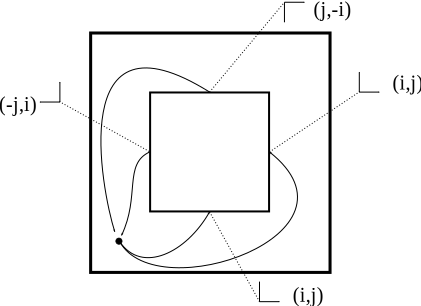
\includegraphics[width=2.9in]{monodromy.png}
\caption{Parallel transporting a unit vector along loops homologous to $c$ and $d$ (left) and corresponding effect $c$ and $d$ loops have on $i,j\in T_{x_0}(\bGs)$ (right).}
\label{fig:loop}
\end{figure}

\begin{thm}
$\varphi_2:\pi_1(\bGs)\rightarrow \mathrm{SO}(2,\ZZ)$ is the rotational monodromy map into $\bGs$'s holonomy group.
\begin{proof}
Let $\gamma:[0,1]\rightarrow\bGs$ be a closed loop on the surface based at $x_0$, and $\alpha\in\pi_1(\bGs,x_0)$ its homotopy class. $\alpha$ is a word in $\<a,b,c,d\>$, so it suffices to show how the vector field along each loop acts on $T_{x_0}$. Because $\bGs$ is flat, trivial loops act trivially on $T_{x_0}$. From figure [??], we can tell this is true of classes $c$ and $d$. Similarly, parallel transportation of a vector field along an element of $a$ or $b$ acts trivially. Since this holds for its generators, it holds for $\alpha$ as well.
\end{proof}
\end{thm}


\begin{lem}
Let $\alpha\in\pi_1(\bGs)$, and let $\gamma:[0,1]\rightarrow\bUs$ be a $u_0$ based homotopy lift into $\btUs$. Then $P_{\gamma}=I_2$ if and only if $\varphi_2(\alpha)=I_2$.
\begin{proof}
Suppose $P_{\gamma}=I_2$. Then $T_{\gamma(0)}(\bUs)=T_{\gamma(1)}(\bUs)$. Since \\\\
FINISH THIS\\\\\\
\end{proof}
\end{lem}



\begin{Def}
Let $\bMs$ be the regular cover of $\bGs$ with deck group $\SO(2,\ZZ)$. Let $p_2:\bMs\rightarrow\bGs$ be the projection of this cover that induces a monomorphism $p_{2*}:\pi_1(\bMs,\xtild)\rightarrow\pi_1(\bGs,x_0)$ such that $p_{2*}\pi_1(\bMs,\xtild)=\ker\varphi_2$.
\end{Def}

\begin{figure}[H]
\centering
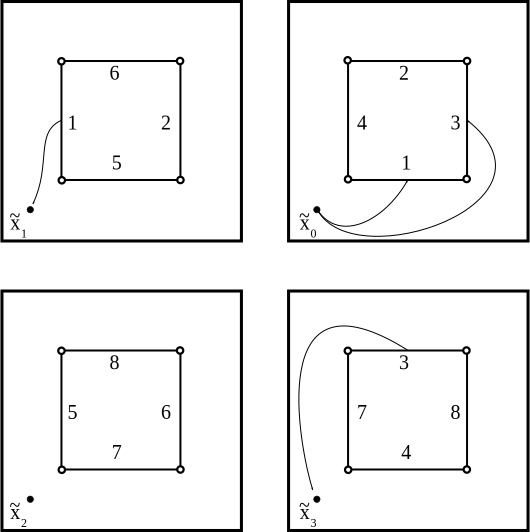
\includegraphics[width=3in]{monogroup.png}
\label{fig:arbitrarylift}
\caption{Lift of paths $c,d$ to $\bMs$}
\end{figure}
The surface $\bMs$ is a degree four cover of $\bGs$ that forces its loops to have trivial rotational holonomy. The metric completion of $\bMs$ is the compact translation surface $\bM$ obtained by reinserting its cone singularities. A \emph{translation surface} is a topological surface with a discrete set of cone singularities and a maximal translation atlas on the surface with these singularities removed. Neighborhoods of the surface are naturally isometric to $\CC$, and a metric on the translation surface is obtained by pulling back $\CC$'s Euclidean metric. We later use $\bMs$ to show that a geodesic in a rational direction on $\bGs$ closes and is unique.


\subsection{A Four-Fold Cover}
We now take these covers we built to construct a third one that covers them all. This is a four-fold cover of $\bUs$ and a $\ZZ^2$ translation cover of $\bMs$ with important properties that allow us to study geodesics on $\bUs$.
\begin{Def}
Let $\btUs$ be the regular cover of $\bUs$ with fundamental group $\pi_1(\btUs)$ and covering map $q_1:\btUs\rightarrow\bUs$ that induces a monomorphism between their fundamental groups such that $q_{1*}\pi_1(\btUs)=\ker\varphi_2\vert_{\ker\varphi_1}$.
\end{Def}


It follows that $\ker\varphi_2\vert_{\ker\varphi_1}=\ker\varphi_1\vert_{\ker\varphi_2}$ since they are taken to abelian groups, and that $\btUs$ is a cover of $\bMs$ as well. We call this projection $q_2:\btUs\rightarrow\bMs$, where it induces a monomorphism such that $q_{2*}\pi_1(\btUs)=\pi_1(\bMs)$.

\begin{thm}
Let $\varphi=\varphi_1\times\varphi_2:\pi_1(\bGs)\rightarrow\ZZ^2\times\SO(2,\ZZ)$. Then $\varphi$ is surjective, and the deck group of the cover $(p_1\circ q_1):\btUs\rightarrow\bGs$ is isomorphic to $\ZZ^2\times\SO(2,\ZZ)$.
\begin{proof}
This follows from the surjectivity of $\varphi_1$, and $\varphi_2$ as generators of both co-domains are mapped to. Since these are compositions of regular covers, $\btUs$ is a regular cover of $\bGs$. The sets of loops that lift to closed curves on $\btUs$ must close on both $\bMs$ and $\bGs$ and their homotopy classes have to belong to the kernel of both homomorphisms. As such, they would belong to the kernel of $\varphi$ as well. Therefore, $\pi_1(\bGs)/(p_{1*}\circ q_{1*})\pi_1(\btUs)=\pi_1(\bGs)/(p_{2*}\circ q_{2*})\pi_1(\btUs)=\varphi(\pi_1(\bGs))=\ZZ^2\times\SO(2,\ZZ)\cong \text{Deck}_{p_1\circ q_1}(\btUs)$.
\end{proof}
\end{thm}

\compav{Might remove this:}

\begin{figure}[H]
\centering
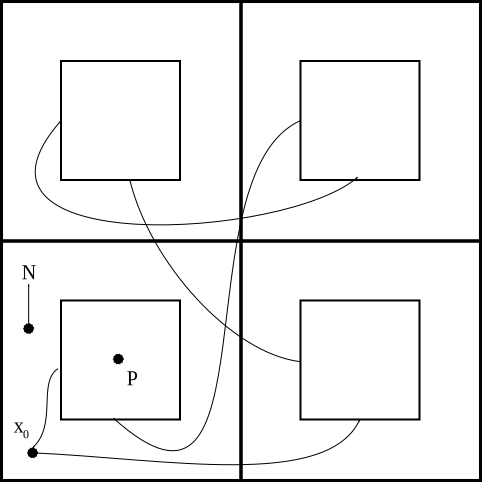
\includegraphics[width=2in]{overlay.png}
\end{figure}

\noindent If we lift this curve to $\btUs$ we can identify it with an element of the deck group, and check if its lift from $\bGs$ belongs to the kernel of both $\varphi_1$ and $\varphi_2$. Fix a direction on this surface pointing north that respects $\bUs$'s compass and rotate every plane by either $90^\circ,$ $180^\circ,$ or $270^\circ$ as the curve travels from one plane (copy of $\mathbf{P}$) to the next. Observe that it will not only close if the curve acts trivially on the holonomy of $\bUs$, but with this construction we can see that $\btUs$ is actually an infinite-type translation surface:

\begin{figure}[H]
\centering
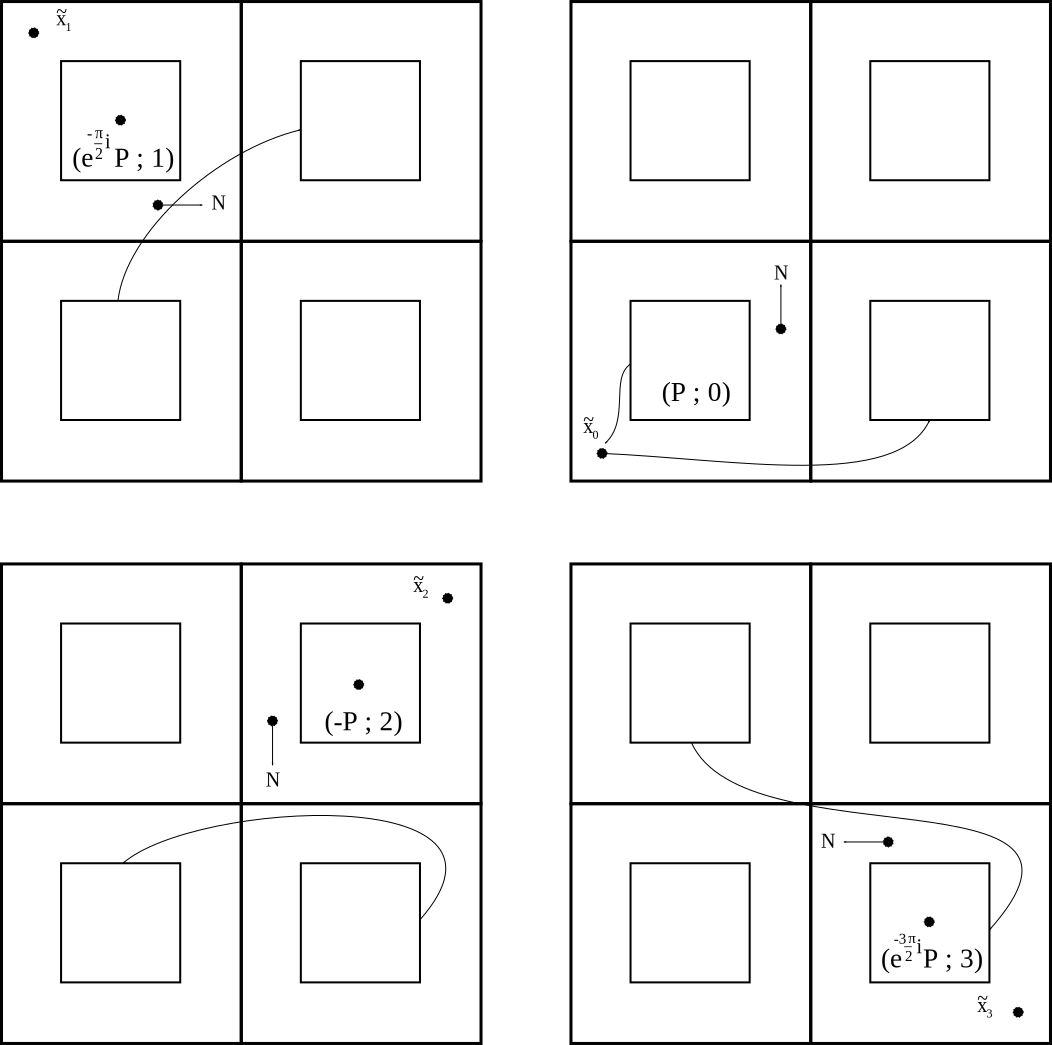
\includegraphics[width=3in]{coverdirection.png}
\caption{With $P\in 2\ZZ+2\ZZ i$.}
\end{figure}

\noindent 

\subsection{Geodesics on $\bUs$}
The key connection made between surfaces $\bUs$ and $\btUs$ is that geodesics on $\bUs$ and $\btUs$ behave identically. For us, a \emph{geodesic}, $\gamma$, is a \emph{unit-speed} locally distance minimizing curve on a smooth surface as a continuous function parameterized by an element in $\RR$. A \emph{geodesic segment} is a restriction of the geodesic to some closed interval in $\RR$. $\gamma$'s derivative is an element of $\RR^2$ in the tangent space at time $t$, denoted $\gamma'(t)\in T_{\gamma(t)}$. To avoid confusion, we say a geodesic segment is \emph{closed} if it returns to the initial point with the same derivative. Otherwise it may self-intersect in a different direction. If the vector can be scaled by $k\in\RR$ such that $kv_0\in\cS$ (defined in the introduction), the geodesic has a \emph{rational} initial trajectory angle. For example, the following is a periodic geodesic on the surface with initial direction $kv_0=(51,31)\in\cO$:
\begin{figure}[H]
\centering
\includegraphics[width=4in]{closed2.png}
\caption{Closed geodesic on $\bUs$ modeled with sage-flatsurf.}
\label{fig:complicated}
\end{figure}
This is in fact the same geodesic as in Figure [??]. When flattened out, it becomes evident that once a choice of angle has been made, there are only four possible directions (when viewed locally) this path can travel in.


\begin{Def}
Let $\rho_t:\RR\rightarrow\bGs$ be a unit-speed geodesic on the \emph{Necker cube surface} with $\rho(0)=x_0$ and $\rho'(0)=v_0$.\\
Let $\Phi_t:\RR\rightarrow\bUs$ be a unit-speed geodesic on the \emph{Necker cube surface} with $\Phi(0)=u_0$ and $\Phi'(0)=v_0$. \\Similarly, let $\tilde{\Phi}_t:\RR\rightarrow\btUs$ be a unit-speed geodesic on $\bUs$'s four-fold cover with $\phitild(0)=\utild$ and $\phitild'(0)=v_0$.\\
Here $u_0$ is a fixed point in $p_1^{-1}(x_0)$ and $\utild$ is a fixed point in $q_1^{-1}(u_0)$. $v_0\in\RR^2$ is a unit-vector in the tangent spaces $T_{x_0}$, $T_{u_0}$, and $T_{\utild}$.
\end{Def}

\begin{thm}[Existence of Rational Closed Geodesics on $\bGs$]
Let $\rho_t:\RR\rightarrow\bGs$ be a geodesic with $k\rho'(0)\in\cS$ for some $k\in\RR$. Then $\rho$ is periodic.
\begin{proof}
Let $\rho_(0)=x_0$. Let $m_0\in p_2^{-1}(x_0)\subset\bMs$, and $\tilde{\rho}_t$ be a geodesic on $\bMs$ based at $m_0$ with derivative $\rho'(0)$ lifted from $\rho$. Since $\bMs$ is a square-tiled translation surface, it is obtainable as the cover of a square torus ramified over a single point. [Veech dichotomy] Therefore the surface is Veech, and $\tilde{\rho}_t$ is either periodic or uniquely ergodic. The initial angle is rational, so it must close. Since it closes on $\bMs$, it must close on $\bGs$ as well.
\end{proof}
\end{thm}

Since $\rho_t$ is periodic, we will denote its restriction to a single period by $\eta(t)=\rho\vert_{[0,T]}(t)$ for $T\in\RR^+$. Here $\eta$ is a closed geodesic segment that returns with the same derivative.

\begin{thm}
Let $\eta$ be as above. Let $\alpha\in\pi_1(\bGs)$ be its homotopy class representative. Then the following is true:
\begin{enumerate}
\item $\Phi(t+T)=\varphi_1(\alpha)\cdot\Phi(t)$ for all $t\in\RR$
\item $\phitild(t+T)=\varphi(\alpha)\cdot\phitild(t)$ for all $t\in\RR$.
\end{enumerate}
\begin{proof}
Let $\tilde{\alpha}$ be a lifted geodesic segment on $\bUs$ based at $u_0$ such that $p_1(\tilde{\alpha}([0,T]))=\eta([0,T])$. Let $\tilde{\tilde{\alpha}}:\RR\rightarrow\bUs\times\ZZ$ be defined as $\tilde{\tilde{\alpha}}(t)=(\alpha^n\cdot\tilde{\alpha}(t~(mod~T)),n)$, where $n=\left\lfloor \frac{t}{T}\right\rfloor$ and $\alpha$ acts by $\varphi_1(\alpha)\in\ZZ^2$. Let $\iota:\bUs\times\ZZ\twoheadrightarrow\bUs$ be the projection given by $(x,z)\mapsto x$. By induction on $\ZZ$, we can show this is a path that extends to the real numbers and that, by uniqueness of geodesics on manifolds, $\iota\circ\tilde{\tilde{\alpha}}=\Phi(t)$. Therefore, $\Phi(t+T)=\alpha^{n+1}\cdot\tilde{\alpha}((t+T)~(mod~T))=\alpha\alpha^n\cdot\tilde{\alpha}(t~(mod~T))=\alpha\cdot\Phi(t)$. \\
The extension to $\RR$ for $\tilde{\Phi}$ is done the same way, and the proof in that case is analogous.
\end{proof}
\end{thm}

\begin{lem}
Let $\alpha,\eta$ be as above. Then $\varphi_2(\alpha)=I_2$.
\begin{proof}
Otherwise $\eta$ would not be a geodesic.
\end{proof}
\end{lem}

\begin{cor}
Let $\alpha$ be as above. If $\varphi_1(\alpha)\neq 0$, then $\Phi$ and $\phitild$ are drift-periodic.
\begin{proof}
Since $\varphi_1(\alpha)$ is isomorphic to an element $f_\alpha\in\text{Deck}_{p_1}(\bUs)$, we need only show that $f_\alpha$ is a local diffeomorphism of $\bUs$. But that much is obvious as neighborhoods are isometric to $\RR^2$ on its smooth sections and $p_1\circ f_\alpha=p_1$. Since $f_\alpha$ is a diffeomorphism, 
\compav{not sure how to do this}
\end{proof}
\end{cor}

\begin{cor}
Let $\alpha$, $\eta$ be as above. Then following are equivalent:
\begin{enumerate}
\item $\Phi$ is periodic.
\item $\phitild$ is periodic.
\item $\varphi(\alpha)=(0,0)$.
\end{enumerate}
\begin{proof}
Suppose $\Phi$ is periodic. Then $\Phi\vert_{[0,T]}$ is a closed segment with trivial holonomy lifted from $\eta$. Let $\alpha\in\pi_1(\bGs)$ be the homotopy class of $p_1(\Phi)=\eta$. From theorems [??] and [??], and lemma [??], $\varphi(\alpha)=((0,0),I_2)$ and so $\phitild(t+T)=\varphi(\alpha)\cdot\phitild(t)=\phitild(t)$ for all $t\in\RR$.\\
Now suppose $\phitild$ is periodic. Then $\varphi_1(\alpha)=(0,0)$ since $\varphi(\alpha)$ is trivial.\\ Now suppose $\varphi(\alpha)=(0,0)$. Then $\Phi(t+T)=\Phi(t)$ for all $t\in\RR$, and so $\Phi$ is periodic.
\end{proof}
\end{cor}

\begin{cor}
Let $\alpha$, $\eta$ be as above. The following are equivalent:
\begin{enumerate}
\item $\Phi$ is drift-periodic.
\item $\phitild$ is drift-periodic.
\item $\varphi_1(\alpha)\neq(0,0)$.
\end{enumerate}
\begin{proof}
Suppose $\Phi$ is drift-periodic. Then $p_1(\Phi\vert_{[0,T]})=\eta$ belongs to $\alpha\in\pi_1(\bGs)$ with $\varphi_1(\alpha)\neq (0,0)$, and so from theorem [??] $\phitild$ is drift-periodic.\\ 
Now suppose $\phitild$ is drift-periodic. From lemma [??], we have that $\phi_2(\alpha)=I_2$. Therefore, $\phi_1(\alpha)\neq (0,0)$ or else $\phitild$ would be closed.\\
Suppose $\varphi_1(\alpha)\neq (0,0)$. Then $\varphi_1(\alpha)$ induces some nontrivial local diffeomorphism $f_\alpha\in\text{Deck}_{p_1}(\btU)$ such that $\Phi(t+T)=\varphi_1(\alpha)\cdot\Phi(t)=f_\alpha(\Phi(t))$ for all $t\in\RR$, and the geodesic drifts by some constant automorphism of the surface.
\end{proof}
\end{cor}



\begin{Def}
Let $\tildphi:\RR\rightarrow\btU$ be a geodesic on the unpunctured four-fold surface such that $\tildphi(0)=\utild$ and $\tildphi'(0)=v_0$.
\end{Def}

\begin{thm}
$\tildphi$ is periodic if and only if $\phitild$ is periodic.\\
$\tildphi$ is drift-periodic if and only if $\phitild$ is drift-periodic.
\end{thm}

This follows readily from the fact that geodesics are undefined on cone singularities. A geodesic on $\btUs$ can be mapped bijectively to a geodesic on  $\btU$ and vice-a-versa. Any automorphisms of $\btU$ can be restricted to $\btUs$, and the notions of periodicity/drift-periodicity of the geodesics are equivalent.



\subsection{Translation Surface}
The surface $\bMs$ was obtained as a cover of $\bGs$ from the rotational monodromy map on $\pi_1(\bGs)$. $\bM$ is its metric completion by reinsertion of its cone singularities. There are four cone singularities on this surface, as opposed to the three on $\bG$, each of cone angle $6\pi$. The individual sections of $\bM$, labeled $I,II,III,$ and $IV$ are rotated in such a way to make it evident that this is indeed a translation surface. (Fig ??) We call the maximal translational $\bM$ atlas $\cA$. Though not immediately apparent, $(\bM,\cA)$ is a square-tiled origami surface. (Fig ??)

\begin{figure}[H]
\centering
\includesvg[width=2.9in]{mtildabw}
\caption{Compact translation surface, $\mathbf{M}$ with edges and cone singularities (1,2,3,4) identified. The Roman numerals are meant to identify every ``copy" of $\bG$ with a vector differing from $v_0$ by rotation of some element in $\SO(2,\ZZ)$. The individual copies are then rotated so that every edge identification is made by translation.}
\label{fig:mtilda}
\end{figure}

\begin{figure}[H]
\centering
\includesvg[width=3.8in]{mtildastaircasebw}
\caption{The staircase surface with roman numerals identifying each section of $\bGs$ in the cover. Edges and cone singularities are labeled. All edges are paired by translation. Two adjacent squares have opposite edges (A through M) identified.}
\label{fig:staircase}
\end{figure}

The lines contained in the squares are the outermost edges in the original image and play an important role in determining the cover, $\btU$. We will orient $\bM$ so that the orientation of its image in $\CC$ under $\cA$ is respected. An orientation preserving affine diffeomorphism of $\bM$ has a derivative in $\CC$ uniform throughout the surface as an element of $\SL(2,\RR)$. The set of these affine diffeomorphisms form the group $\text{Aff}_+(\bM)$. The map $D:\text{Aff}_+(\bM)\rightarrow\SL(2,\RR)$ factors through $\cA$ and is a homomorphism between these groups. The affine group's image in $\SL(2,\RR)$ is itself a subgroup known as the \emph{Veech group} of $\bM$, which we denote $V(\bM)$. If $V(\bM)$ is of finite index in $\SL(2,\RR)$, we say that $\bM$ is a \emph{Veech surface}. A theorem of Gutkin-Judge states that any compact, square-tiled translation surface is in fact Veech. $\bM$  has am obvious construction as a branch cover of the square torus, ramified over a single point.\\

\noindent There are two transverse cylinder decompositions of this surface in vertical and horizontal directions. In each decomposition, there are is a cylinder waist curve running along the circumference of the cylinder. We use $\gamma_i$ to indicate which waist curve we are referring to. (Fig [??])

\begin{figure}[H]
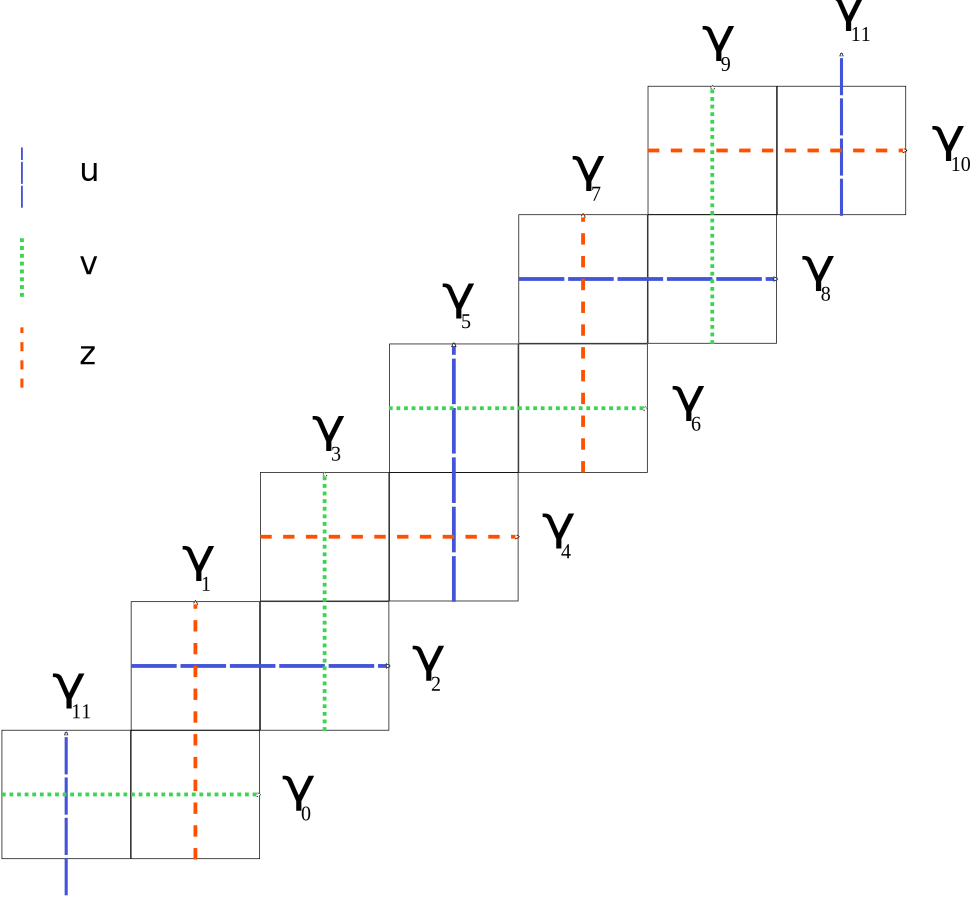
\includegraphics[width=4in]{homologyclass.png}
\centering
\caption{$\bM$'s waist curves with u,v, and z homology class labels.}
\label{fig:homology}
\end{figure}

We will use the first homology of the surface, $H_1(\bM,\QQ)$, to determine the cover. These curves associate an even indexed waist curve with a horizontal cylinder and an odd indexed waist curve with a vertical cylinder, a construction that becomes useful later on. Let $[\gamma_i]\in H_1(\bMs,\QQ)$ be the homology class corresponding to $\gamma_i$. We use $\Gamma=\{[\gamma_i]~:~0\leq i \leq 11\}$ to denote the set of these classes.

\begin{Def}
The homology classes $u,v,z$ are given as the following weighted sums of elements of $\Gamma$:
\begin{align*}
u &= -[\gamma_2] +[\gamma_5] + [\gamma_8] - [\gamma_{11}],\\
v &= +[\gamma_0] -[\gamma_3] -[\gamma_6] +[\gamma_9],\\
z &= +[\gamma_1] +[\gamma_4]-[\gamma_7]-[\gamma_{10}].
\end{align*}
\end{Def}

\begin{Def}
Algebraic intersection number on a differentiable, orientable manifold is an integer value obtained as a scalar product of two elements in its first homology.
\begin{align*}
\<\<\cdot~,~\cdot\>\>:H_1(\bM,\QQ)\otimes H_1(\bM,\QQ)\rightarrow\ZZ
\end{align*}
Let $\alpha,\beta$ be two closed curves on $\bM$, and let $\overline{\alpha},\overline{\beta}$ be their respective homology classes. For $\overline{\alpha},\overline{\beta}\in H_1(\mathbf{M},\QQ)$, $\<\<\alpha,\beta\>\>$ returns the signed intersection number of two homology classes as a sum of intersections of the two curves, where  an intersection is positive (+1) if $\beta$ makes a positive angle relative to the direction $\alpha$ is traveling in. A crossing is negative (-1) if $\beta$ makes a negative angle relative to $\alpha$. $\bM$ is oriented so thats its image in $\CC$ under translational charts agrees with the orientation of $\CC$.
\end{Def}

It's known that the intersection number is a non-degenerate, bilinear form. We use this fact to find a basis for $H_1(\bM,\QQ)$.

\begin{lem}
$\Gamma$ generates $H_1(\bM,\QQ)$.
\begin{proof}
Let $E_{i,j}:=\<\<[\gamma_j],[\gamma_i]\>\>$ for $i,j\in \{0,1,2,\cdots,11 \}$. $E$ is an intersection matrix of rank 10. Since intersection number is non-degenerate, $\Gamma$ must span all of $H_1(\bM,\QQ)$.
\end{proof}
\end{lem}

\begin{cor}
The set $\Gamma'=\Gamma\backslash\{[\gamma_7],~[\gamma_{10}] \}$ forms a basis for $H_1(\bM,\QQ)$. Further,
\begin{align}
[\gamma_7]&=[\gamma_1]-[\gamma_3]+[\gamma_5]+[\gamma_9]-[\gamma_{11}],\\~and~
[\gamma_{10}]&=[\gamma_0]-[\gamma_2]+[\gamma_4]-[\gamma_6]+[\gamma_8].
\end{align}
\begin{proof}
Let $M_{i,j}:=\<\<[\gamma_j],[\gamma_i]\>\>$ for $i,j\in \{0,1,2,\cdots,11 \}\backslash\{7,10\}$. Then $\det M=10$, proving the first statement. \\\\Now since intersection is  non-degenerate, if we intersect $[\gamma_7]$ and $[\gamma_{10}]$ with $\sum\Gamma$, a spanning set of $H_1(\bM,\QQ)$, we obtain $\<\<\sum\Gamma,[\gamma_7]\>\>=$\\\\
(Might not use (5) and (6)).\\\\
To prove the second claim it suffices to show that passing the RHS of (5) and (6) through the matrix $E_{i,j}$ will equate them to $[\gamma_7]$ and $[\gamma_{10}]$ respectively.
\end{proof}
\end{cor}

\begin{cor}
The sets $u$ and $v$ are linearly independent.
\begin{proof}
Obviously follows.
\end{proof}
\end{cor}

\begin{Def}
Fix $m_0\in\bMs$ and let $\beta\in\pi_1(\bM,m_0)$. The map $\Omega_{u,v}:\pi_1(\bM)\rightarrow \ZZ^2$ is given as
\begin{align*}
\Omega_{u,v}([\beta])=(~\<\<u,\beta\>\>~,~\<\<v,\beta\>\>~)
\end{align*}
\end{Def}

This homomorphism takes $\pi_1(\bM)$ to an abelian group, so it can be factored through $H_1(\bM,\QQ)$, and a cover of $\bM$ is obtained from the kernel of this map. This is a special case when it comes to regular covers with abelian Deck groups.

\begin{thm}
Let $\pi_1(\btU,\utild)$ be the fundamental group of $\btU$ with $\utild\in (q_1\circ p_1)^{-1}(x_0)$ and $x_0\in\bGs$, and $m_0\in p_2^{-1}(x_0)$. Let $p_r:\btU\twoheadrightarrow\bM$ be a projection of surfaces by taking a $\ZZ^2$ quotient of its translational symmetries. Then $p_r$ induces a map $p_{r*}:\pi_1(\btU,\utild)\rightarrow\pi_1(\bM,m_0)$ such that $p_{r*}\pi_1(\btU)=\ker\Omega_{u,v}$.
\begin{proof}
The curves making up $u$ and $v$ are the outermost edges of sections $I,~II,~III,~IV$. (Fig 9) By observation, these classes are determined and weighted according to which section in the fiber over $\bM$ a lifted path ends up on after a positive or negative crossing.\\\\\\
Might need to redo this, factor through null space of $\Omega$ matrix.
\end{proof}
\end{thm}

\subsection{Induced Automorphisms of $H_1(\bM,\QQ)$}
We have previously remarked on the uniformity of $\bM$'s cylinder decompositions, $\mathfrak{H},~\mathfrak{V}$, but have yet to show the correlation between these cylinders and $\text{Aff}^+(\bM)$. We say the \emph{modulus}, $\mu_i$, of the cylinder containing the $i^{th}$ waist curve is the ratio of its width to its circumference, $\frac{w_i}{c_i}$. The $\emph{Dehn-twist}$ of a cylinder in either set is an affine diffeomorphism that skews the cylinder and preserves edges and vertices. The skew is in the direction of the waist curve.

\begin{figure}[H]
\centering
\includesvg[width=3in]{cylinderskew}
\label{fig:skew}
\caption{Dehn-twist of a cylinder in $\bM$'s horizontal cylinder decomposition.}
\end{figure}

In local coordinates this Dehn-twist has derivative $\left[~\begin{matrix}1 && \pm\mu_{2i}^{-1}\\0 && 1\end{matrix}~\right]$. On $\bM$ the cylinders in both vertical and horizontal decompositions have moduli $\mu_i=\frac{1}{2}$. Dehn-twists on $\mathfrak{H}$ and $\mathfrak{V}$ give up global diffeomorphisms as $\emph{multi-twists}$ of $\bM$ with the same derivatives. [cite] 

\begin{Def}
We denote the global affine diffeomorphisms of $\text{Aff}^+(\bM)$ obtained as \textbf{multi-twists} of the surface in \textbf{horizontal and vertical directions} $\psi_h$ and $\psi_v$, respectively.
\end{Def}

The images of the twists $\psi_h$ and $\psi_v$ under the derivative map $D$ are taken to the same matrices as the Dehn-twists in local coordinates. i.e.
\begin{align*}
D(\psi_h)=\psi_h'=\left[ \hspace{1mm} \begin{matrix}
				1 &   2\\
				0 & 1
			\end{matrix}\hspace{1mm}\right] \hspace{0.5in}
			D(\psi_v)=\psi_v'=\left[ \hspace{1mm} \begin{matrix}
							1 & 0\\
							 2 & 1
						\end{matrix}\hspace{1mm}\right]
\end{align*}

These are parabolic elements of $V(\bM)$ that generate a free group of rank 2. [cite].
\begin{Def}
Let $\XX$ be the generated parabolic subgroup of $\text{Aff}^+(\bM)$, where $\XX=\<\psi_h,\psi_v \>$.
\end{Def}

The image of this group under $D$ is itself a subgroup of $V(\bM)$, $\XX'=D(\XX)=D(\<\psi_h,\psi_v \>)=\<D(\psi_h),D(\psi_v)\>=\<\psi_h',\psi_v' \>$. When skewing the surface and piecing it back together under $\psi_h$ or $\psi_v$, the cylinder curves intersect each other in pairs:

\begin{figure}[H]
\centering
\includesvg[width=2in]{skew}
\end{figure}

By skewing in the horizontal direction, $\psi_h$ preserves the even indexed cylinder curves, but the odd indexed vertical curves $\gamma_i$ intersect the two horizontal curves (positive intersection), $\gamma_{i-1}$ and $\gamma_{i+1}$. A similar observation can be made from applying $\psi_v$, where the vertical curves are preserved but the horizontal curves intersect with adjacent vertical curves (negative intersection). Let $\Aut(H_1(\bM,\QQ))$ be the group of automorphisms of $\bM$'s homology. By extension of these affine maps to the automorphism group, we may express the \emph{induced} automorphisms as they affect the homology generating set $\Gamma$. In turn, these automorphisms act linearly on a cycle $\mathfrak{c}=\sum_{i=0}^{11}k_i[\gamma_i]\in H_1(\bM,\QQ)$. Let $i\in\ZZ/12\ZZ$. Then the following formulas hold for $\psi_h$ and $\psi_v$'s counterparts in $\Aut(H_1(\bM,\QQ))$ raised to $k\in\ZZ$:

\begin{align*}
\psi^{*k}_h([\gamma_i])=&[\gamma_i] + \frac{k}{2}(1-(-1)^i)([\gamma_{i-1}]+[\gamma_{i+1}])\\
\psi^{*k}_v([\gamma_i])=&[\gamma_i] - \frac{k}{2}(1+(-1)^i)([\gamma_{i-1}]+[\gamma_{i+1}])\\
\end{align*}

These are used to generate the group $\XX^*=\<\psi^{*}_h,\psi^{*}_v \>$. There are no relations between its generators since $i$, being either even or odd, has one automorphism act trivially while the other acts non-trivially. Therefore this group is also a free group of rank 2. All of our related groups are rank 2 free groups, so they are isomorphic.


Let $\tau\in\XX$. Let $D(\tau)=\tau'\in\XX'$ and $\tau^*\in\XX^*$ be $\tau$'s isomorphic counterparts in their respective groups. We say $\tau=\prod_{j=0}^{n}\psi_h^{k_j}\circ\psi_v^{m_j}$ is a word in $\XX$ as a finite left concatenated product of multi-twist pairs with $k_j,m_j\in\ZZ$. Let $\psi_j=\psi_h^{k_j}\circ\psi_v^{m_j}$ be the $j^{th}$ multi-twist pair. Since $\tau',\tau^*$ are isomorphic, we can use these expressions interchangeably. \\\\
The corresponding $j^{th}$ automorphism pair is an element $\psi_j^*\in\Aut(H_1(\bM,\QQ))$ and is expressed as 

\begin{align*}
\psi_j^*([\gamma_i])=&[\gamma_i]+\frac{k_j(1-(-1)^i)}{2}([\gamma_{i-1}]+[\gamma_{i+1}])\\&-\frac{m_j(1+(-1)^i)}{2}(k_j(2[\gamma_i]+[\gamma_{i-2}]+[\gamma_{i+2}]) +[\gamma_{i-1}]+[\gamma_{i+1}]).
\end{align*}

\noindent Similarly,

\begin{align*}
\psi_j'=\left[ \hspace{1mm} \begin{matrix}
				1 &   2\\
				0 & 1
			\end{matrix}\hspace{1mm}\right]^{k_j}\left[ \hspace{1mm} \begin{matrix}
							1 &   0\\
							2 & 1
						\end{matrix}\hspace{1mm}\right]^{m_j}=\left[ \hspace{1mm} \begin{matrix}
										1+4m_jk_j &   2k_j\\
										2m_j & 1
									\end{matrix}\hspace{1mm}\right].
\end{align*}


\noindent Let $\sum\Gamma=\sum_{i=0}^{11}[\gamma_i]$, and denote the odd and even indexed sums of homological waist curves $\sum\Gamma_o$ and $\sum\Gamma_e$, respectively. We look at three kinds of closed geodesic segments on $\bM$, not considering initial/terminal points for the time being. These are the geodesics in directions $\theta=0,~\frac{\pi}{2},$ and $\frac{\pi}{4}$. The aim is to show that these linear automorphisms take $\sum\Gamma\mapsto c_1\sum\Gamma_e+c_2\sum\Gamma_o$, and acts faithfully on the kernel of $\Omega_{u,v}$. \\



\noindent Let $\chi$ be the geodesic segment in direction $\theta=\frac{\pi}{4}$ that runs up the staircase intersecting every $\gamma_i$ exactly once. Denote its homology class $[\chi]$. If we flow $\bM$ in this direction we obtain a two cylinder decomposition of the surface, where $\chi$ is contained in or the other cylinder.
\begin{figure}[H]
\centering
\includesvg[width=5.9in]{slopeonecylinder}
\caption{Cylinder decomposition with $[\chi]$ being the dashed or dotted geodesic. $[\chi]$ is homologous to $\frac{1}{2}\sum\Gamma$ (solid/curvy)}
\end{figure}
Observe from the previous figure that $\chi$ is homologous to $\frac{1}{2}\sum\Gamma$, a curve that climbs up the staircase by traversing each waist curve exactly halfway ( their intersection number is 0). When lifted to $\btU$ and projected onto $\bUs$, this is a closed geodesic on the Necker cube surface (Fig 1).


\begin{lem}
$\Omega_{u,v}([\chi])=(0,0).$
\begin{proof}
Consider $\Omega_{u,v}([\chi])=\Omega_{u,v}(\frac{1}{2}\sum\Gamma)=\frac{1}{2}(i(u,\sum\Gamma),i(v,\sum\Gamma))$. \\Since only adjacent curves intersect,\\ $i(u,\sum\Gamma)=i(-[\gamma_2],[\gamma_{1}]+[\gamma_{3}]) +i([\gamma_5],[\gamma_{4}]+[\gamma_{6}]) + i([\gamma_8],[\gamma_{7}]+[\gamma_{9}]) - i([\gamma_{11}],[\gamma_{10}]+[\gamma_{0}])\\=-2+(-2)+2-(-2)=0$.\\
Similarly,\\ $i(u,\sum\Gamma)=i([\gamma_0],[\gamma_{11}]+[\gamma_{1}]) -i([\gamma_3],[\gamma_{2}]+[\gamma_{4}]) -i([\gamma_6],[\gamma_{5}]+[\gamma_{7}]) +i([\gamma_9],[\gamma_{8}]+[\gamma_{10}])\\=2-(-2)-2+(-2)=0$. Therefore, $\Omega_{u,v}([\chi])=(0,0)$.
\end{proof}
\end{lem} 
Since $\chi$ is homologous to this sum of waist curves divided by two, there's a bit of freedom in how we can express a cycle in the orbit of $[\chi]$ in $H_1(\bM,\QQ)$ by seeing how an element in $\XX^*$ acts on $\sum\Gamma$.

\begin{lem}
Let $\tau\in\XX$. If $\alpha=\tau(\chi)$ is a closed geodesic segment on $\bM$, then $[\alpha]=\frac{1}{2}(c_1\sum_e+c_2\sum_o)$ for $c_1,c_2\in\ZZ$.
\begin{proof}(By Induction on $\psi^*_j\in\XX^*$).\\
Consider $\psi_0(\chi)$.\\
$[\psi_0(\chi)]=\psi_0^*([\chi])=\frac{1}{2}\psi_0^*(\sum\Gamma)=\frac{1}{2}\psi_0^*(\sum\Gamma_e+\sum\Gamma_o)=\frac{1}{2}(\psi_0^*(\sum\Gamma_e)+\psi_0^*(\sum\Gamma_o))$. \\Now $\psi_0^*(\sum\Gamma_e)\\=\sum_{i=0}^{11}\psi_0^*([\gamma_{2i}])\\=\sum_{i=0}^{11}( [\gamma_{2i}]-2m_0k_0[\gamma_{2i}]-m_0k_0[\gamma_{2i-2}] -m_0k_0[\gamma_{2i+2}]-m_0[\gamma_{2i+1}]-m_0[\gamma_{2i-1}] )\\=(1-4m_0k_0)\sum\Gamma_e+(-2m_0)\sum\Gamma_o$.\\
Similarly,\\ $\psi_0^*(\sum\Gamma_o)\\=\sum_{i=0}^{11}\psi_0([\gamma_{2i+1}])=\sum_{i=0}^{11}([\gamma_{2i+1}] +k_0([\gamma_{2i}]+[\gamma_{2i+2}]))\\=\sum\Gamma_o+2k_0\sum\Gamma_e$.\\
And so,\\ $\frac{1}{2}\psi_0^*(\sum\Gamma)=\frac{1}{2}((1+2k_0-4m_0k_0)\sum\Gamma_e +(1-2m_0)\sum\Gamma_o )$.\\\\
Induction: Suppose $\psi^*_j(\sum\Gamma)=c_1\sum\Gamma_e+c_2\sum\Gamma_o$.\\
Then $\psi^*_{j+1}(\psi^*_{j}(\sum\Gamma))\\=c_1\psi^*_{j+1}(\sum\Gamma_e)+c_2\psi^*_{j+1}(\sum\Gamma_o)\\=
c_1((1-4m_{j+1}k_{j+1})\sum\Gamma_e+(-2m_{j+1})\sum\Gamma_o)+c_2(\sum\Gamma_o+2k_{j+1}\sum\Gamma_e)\\=
(c_1(1-4m_{j+1}k_{j+1}) + 2k_{j+1}c_2)\sum\Gamma_e+(-2m_{j+1}c_1+c_2)\sum\Gamma_o$.\\
Hence, $[\alpha]=\frac{1}{2}(c_1'\sum_e+c_2'\sum_o)$.

\end{proof}
\end{lem}

\begin{thm}
Let $\tau$ be as above. Suppose $\alpha=\tau(\chi)$. Then $\Omega_{u,v}([\alpha])=(0,0)$. 
\begin{proof}
$\Omega_{u,v}([\alpha])=\Omega_{u,v}([\tau(\chi)])=\Omega_{u,v}(\tau^{*}([\chi]))=\frac{1}{2}(i(u,\tau^*(\sum\Gamma)), i(v,\tau^*(\sum\Gamma))$.\\
Now by the previous lemma, \\$i(u,\tau^*(\sum\Gamma)=c_1 i(u,\sum
\Gamma_e)+c_2 i(u,\sum\Gamma_o)$ $\\= c_1(i([\gamma_5],[\gamma_{4}]+[\gamma_6]) - i([\gamma_{11}],[\gamma_{10}]+[\gamma_{0}]))\\+c_2(-i([\gamma_2],[\gamma_{1}]+[\gamma_{3}]) + i([\gamma_8],[\gamma_{7}]+[\gamma_{9}]) )\\=c_1((-2)-(-2))+c_2(-2+ 2 )=0\\$
It's shown similarly that $i(v,\tau^*(\sum\Gamma))=0$.
Therefore $\Omega_{u,v}([\alpha])=(0,0)$.
\end{proof}
\end{thm}

Now we know that $\chi$ serves as something of a basis for a class of lifted closed segments. Because the sums of even and odd curves belong individually in the kernel of $\Omega_{u,v}$, anything in the orbit of $\chi$ will also lift to a closed segment on $\btU$. To show that these are the only segments that lift to closed paths on $\btU$, we look at the orbit of segments in directions $\theta=0$ and $\frac{\pi}{2}$ that are homologous to some $\gamma_{2i}$ and $\gamma_{2i+1}$, respectively. These will then span the rest of the homology classes of closed geodesic segments of $\bM$. 

\begin{lem}
$\Omega_{u,v}([\gamma_i])\neq (0,0)$.
\begin{figure}[H]
\begin{wrapfigure}{l}{2.9in}
\includegraphics[width=2.9in]{12gon.png}
\end{wrapfigure}
~\\\vspace{0.5in}\\Every curve, $\gamma_i$, intersects exactly one adjacently indexed curve that is an element of exactly one of either $u$ or $v$, or with one of both $u$ \emph{and} $v$. The image to the left shows every curves associated image under $\Omega_{u,v}$. Therefore, these classes are always taken to a non-trivial element of $\ZZ^2$ under $\Omega_{u,v}$.
\end{figure}

\end{lem}
\vspace{0.8in}

\begin{lem}
$\left[\begin{matrix}
1 & -1 & 0 & -1 & -1 & 0 & -1 & 0 & 1 & 0\\
0 & 1 & 1 & 0 & 1 & -1 & 0 & -1 & 0 & 1\\
\end{matrix}\right]$. Further its rank is 2 and nullity is 8.
\end{lem}

\begin{thm}
Let $\sigma\in\XX$. Suppose $\beta=\sigma(\gamma_i)$. Let $[\beta]$ be its homology class. Then $\Omega_{u,v}([\beta])\neq (0,0)$.
\begin{proof}
Since $\beta=\sigma(\gamma_i)$, $[\beta]=[\sigma(\gamma_i)]=\sigma^*\cdot[\gamma_i]$. Express $\psi_j^*$ as a $10\times10$ matrix acting on standard basis coefficients of $\Gamma'$. This is a rank 10 matrix. The product $\psi_{j+1}^*\cdot\psi_j^*$ is also a rank 10 matrix. By induction on $j$, $\sigma^*$ is a finite left concatenated product of these matrices and is rank 10 as well. If $[\gamma_i]\in\Gamma'$ it is rank 1. If it is $[\gamma_7]$ or $[\gamma_{11}]$, by [LEM] it is a subspace of $H_1(\bM,\QQ)$ spanned by four other curves. Therefore the rank of $\sigma^*\cdot[\gamma_i]$ is less than or equal to 4. The matrix representation of $\Omega_{u,v}$ on $\Gamma'$ has nullity 8. Therefore $[\beta]$ is in a subspace of dimension always less than the dimension of the kernel of $\Omega_{u,v}$ and so $\Omega_{u,v}([\beta])\neq (0,0)$.
\end{proof}
\end{thm}

Now since $\Omega$ and $\varphi_1$ are maps into abelian groups, they factor through the homology of these surfaces. There is a linear transformation between their homologies that ensures every closed geodesic on both surfaces are taken to the same $\ZZ^2$ element in the cover.



\begin{Def}
Let $\alpha\in H_1(\bM, \QQ)$ with coordinates relative to $\Gamma'$ (order of coefficients still ascending). Let $v_\alpha\in\QQ^{10}$ be the vector of rational coefficients. We use the fact that rational homology is the abelianization and field extension of the free group $\pi_1(\bGs)$ to say an element in $H_1(\bGs,\QQ)$ is of the form $x_1a+x_2b+x_3c+x_4d$. Let $L:H_1(\bM,\QQ)\twoheadrightarrow H_1(\bGs,\QQ)$ be the linear transformation between these vector spaces given by:
\begin{align}
L(\alpha):=\left[\begin{matrix}
1 & -1 & 0 & -1 & -1 & 0 & -1 & 0 & 1 & 0\\
0 & 1 & 1 & 0 & 1 & -1 & 0 & -1 & 0 & 1\\
0 & 1 & 0 & 0 & 0 & 0 & 0 & 0 & 0 & 0\\
0 & 0 & 0 & 0 & 1 & 0 & 0 & 0 & 0 & 0\\
\end{matrix}\right]v_{\alpha}\cdot \left[\begin{matrix}
a \\ b \\ c\\ d\\
\end{matrix}\right]^{\perp}
\end{align}
\end{Def}

A quick calculation shows us that this matrix is rank 4, making $L$ is surjective. 

\begin{thm}
Let $\alpha\in\pi_1(\bGs,x_0)$ be the homotopy class of a closed geodesic segment. Then its lifted image is homotopic to a non-trivial element $\beta\in\pi_1(\bM,m_0)$. Furthermore, these homotopy classes have the property that $\varphi_1(\alpha)=\Omega_{u,v}(\beta)$.
\begin{proof}
Observe that the lifted homotopy  $\tilde{\alpha}\in\pi_1(\bMs,m_0)$ as $\alpha\in\ker\varphi_2$. [lem] Since a periodic geodesic is non-singular, $\tilde{\alpha}$'s unique geodesic can be mapped to the unpunctured surface $\bM$ and vice-versa (where $m_0$ is \emph{not} a cone singularity). Call its homotopy class $\beta$. A geodesic on a compact, orientable hyperbolic surface could not be contracted to a single point. If that were true, the geodesic would have had to have curvature $\pi$ according to the Gauss-Bonnet Theorem, which is a contradiction. Therefore $\beta$ is non-trivial and its homology class has a coordinate $v_{\beta}\in \QQ^{10}$. Since $\varphi_1$ factors through homology, we may write $\varphi_1(\alpha)=\left[\begin{matrix} 1 & 0 & 0 & 0\\0 & 1 & 0 & 0\end{matrix}\right]v_\alpha\in\ZZ^2$. Now if we combine these two we get $\varphi_1\circ L=\left[\begin{matrix}
1 & -1 & 0 & -1 & -1 & 0 & -1 & 0 & 1 & 0\\
0 & 1 & 1 & 0 & 1 & -1 & 0 & -1 & 0 & 1\\
\end{matrix}\right]$ as a function from $H_1(\bM,\QQ)$ to $\ZZ^2$. Let $v_\beta=(k_1,k_2,\cdots,k_{10})$. Now if we pass $\beta$'s abelianized form, $[\beta]$, along to $\varphi_1\circ L$, we have the first coordinate equal to $k_1-k_2-k_4-k_5-k_7+k_9\\
=i(-[\gamma_2],k_2[\gamma_1]+k_3[\gamma_2])+i([\gamma_5], k_6[\gamma_5]+k_5[\gamma_4]+k_7[\gamma_6])\\+i([\gamma_8],k_8[\gamma_8]+k_9[\gamma_9])+i(-[\gamma_{11}],k_1[\gamma_{0}]+k_4[\gamma_3])\\=i(u,[\beta])$.\\
Similarly, the second coordinate is just $i(v,[\beta])$. Thus $\Omega_{u,v}=\varphi_1\circ L$. Since $\alpha$ and $\beta$ are in one-to-one accordance, $L([\beta])=[\alpha]$, which means $\Omega_{u,v}(\beta)=\varphi_1(L([\beta]))=\varphi_1([\alpha])=\varphi_1(\alpha)$.
\end{proof}
\end{thm}

Now projecting back onto the space allows us to identify an element of the deck group by some $\ZZ^2$ action on $\bUs$. 


\section{Proof of Main Theorem}
Existence of an element in $\XX$ that sends a geodesic to one that is homologous to $\chi$ or some waist curve relies on the isomorphic properties of groups $\XX$, $\XX'$, and $\XX^*$. In the end the faithfulness and transitivity of one group implies the faithful action on the kernel of $\Omega_{u,v}$. The following is a well known fact of the group $\XX'$:
\begin{lem}
$\XX'=\ker m$ where $m:M(2,\ZZ)\rightarrow M(2,\ZZ)(mod~2)$.
\end{lem}
This lemma is used primarily to establish faithfulness.
Recall that $(x,y)\in S=\cO\cup \cE$ is an element of $\ZZ^2$ with $x,y$ relatively prime. Further partition $\cE$ into sets $\cE_1$ and $\cE_2$, where integer pairs $(x,y)\in\cE$ are in $\cE_1$ if $x$ is odd or in $\cE_2$ if $x$ is even. These are disjoint since $x$ and $y$ cannot both be even or odd. Let $\XX'$ act on $\cS$ by linear transformations on $\ZZ^2$. In these proofs we make use of Bezout's identity often to establish transitivity on $\cO,\cE_1,$ and $\cE_2$: 

\begin{align}
\text{For any relatively prime }x,y\text{ there exist }m,n\in\ZZ\text{ such that }mx+ny=1.
\end{align}

\subsection{Orbit of Rational Directions}
Here are some results we use in the next section that are used to prove existence of geodesics in any given rational direction.

\begin{lem}
$\XX'$ acts faithfully and transitively on $\cO$.
\begin{proof}
Let $v_0=\begin{pmatrix}x \\ y\end{pmatrix}\in\cO$, where $x,y$ are both odd and relatively prime integers. Let $M=\begin{pmatrix}a & b \\ c & d
\end{pmatrix}\in\XX'$. Let $u=\begin{pmatrix}1 \\ 1 \end{pmatrix}\in\cO$. It follows that this action is faithful since $ax+by$ and $cx+dy$ cannot sum up to an element in $\cE$, as $a,d$ are odd and $b,c$ are even. We show that there is a matrix $M$ such that $Mu=v_0$, i.e. $a+b=x$ and $c+d=y$. We know $\det M=ad-bc=1$ and from $(*)$ that there exist $m,n\in\ZZ$ such that $1=mx+ny$. Let $a=(x-b)$, $b=n(xy-1)$, $c=m(xy-1)$, and $d=(y-c)$. Then
\begin{align*}
\det M&=(x-n(xy-1))(y-m(xy-1))-n(xy-1)m(xy-1)\\
&=xy-mx(xy-1)-ny(xy-1)+mn(xy-1)^2-mn(xy-1)^2\\
&=xy-x^2my-y^2nx+(mx+ny)=xy-xy(mx+ny)+1\\
&=xy-xy+1=1.
\end{align*}
Therefore $M\in\SL(2,\ZZ)$. Now its clear that $a+b=(x-b)+b=x$ and $c+d=c+(y-c)=y$. Further, $b=n(xy-1)$ and $c=m(xy-1)$ are even since $xy-1$ is even, and so $a=x-b$ and $d=y-c$ are odd. Hence, $M\in\ker m$ and $Mu=v_0$. $M$ is invertible, so $M^{-1}v_0=u.$ Apply the same argument for some other $v_0'\in\cO$, and obtain that $N^{-1}v_0'=u.$ We conclude then that $NM^{-1}v_0=v_0'$ for any $v_0,v_0'\in\cO$. Therefore $\XX'$ acts transitively on $\cO$.
\end{proof}
\end{lem}

\begin{lem}
$\XX'$ acts faithfully and transitively on $\cE_1$ and $\cE_2$.
\begin{proof}
Let $v_0=\begin{pmatrix}x \\ y\end{pmatrix}\in\cE$, where $x,y$ are relatively prime integers. Let $M=\begin{pmatrix}a & b \\ c & d
\end{pmatrix}\in\XX'$. Let $u_1=\begin{pmatrix}1 \\ 0 \end{pmatrix}\in\cE_1$ and $u_2=\begin{pmatrix}0 \\ 1 \end{pmatrix}\in\cE_2$.\\\\
Case I: $v_0\in \cE_1$. Then let $a=x$, $b=-n$, $c=y$, and $d=m$, where $mx+ny=1$ by $(*)$.  Then
\begin{align*}
\det M &= ad-bc=xm-(-ny)=mx+ny=1.
\end{align*}
Hence $Mu_1=v_0$, and $M\in\XX'$ since $p(M)=I_2$. Repeating this argument for $v_0'\in \cE_1$, we get that $Nu_1=v_0'$. Therefore, $v_0=MN^{-1}v_0'$ and this action is transitive.\\\\\compav{Dont forget to prove faithfulness.}
Case II: $v_0\in \cE_1$. The proof for this is analogous to the previous case.
\end{proof}
\end{lem}

\subsection{Directions \& Geodesic Orbits}
Let $\hol:H_1(\bM,\QQ)\rightarrow\RR^2$ be the translational holonomy vector map that associates each cycle with a vector in $\RR^2$. The holonomy map preserves distances and is an accurate representation of a geodesic segment on $\bM$. In local coordinates an element of $V(\bM)$ factors through $\hol$. For example $\chi$ is a geodesic segment in direction $\theta=\frac{\pi}{4}$ with $\hol([\chi])=(6,6)$. After applying one multi-twist in the horizontal direction, we obtain $\hol([\psi_h(\chi)])=\hol(\psi_h^*([\chi])=\psi_h'\cdot\hol([\chi])=\psi_h'\cdot(6,6)=(18,6)=6(3,1)$. 

We denote the set of closed non-singular geodesics (separatrices) based at $x\in\bMs$ as $V_{x}$. The collection of these geodesics is the set $\cV=\bigcup_{x\in\bMs} V_{x}$. Let $\tau\in\XX\subseteq \text{Aff}^{+}(\bM)$. Then $\tau$ induces an automorphism of $\cV$ that maps $V_{x}$ to $V_{\tau(x)}$. In addition to this, it is a parabolic isometry of the surface that takes a geodesic in $V_{x}$ in direction $\theta$ to a geodesic in $V_{\tau(x)}$, not necessarily in the same direction. $V_{x}$ forms a set of homology classes, $[V_{x}]$, such that $\hol([V_{x}])$ and $\hol([V_{\tau(x)}])$ are indistinguishable, discrete subsets of $\RR^2$. The faithful, transitive action of $D(\tau)=\tau'$ on $\cO$ and $\cE$ extends to $\hol([V_{x}])$. Because $\tau$ is isometric to $\tau^*\in\XX^*\subseteq \Aut(H_1(\bM,\QQ))$, the relationship between a choice of direction of a given geodesic, $\alpha$, based at $m_0$ and the orbit of its homology class becomes clear.

\begin{Def}
Let $\phi_t^\theta:\RR\rightarrow\bM$ be a unit-speed geodesic with base point $m_0$ in direction $\theta\in \RR/2\pi\ZZ$. Let $v_\theta=(\cos\theta,\sin\theta)\in\RR^2$ be a unit-vector in direction $\theta$. If this direction is rational, then $v_\theta$ is scaled by some $k\in\RR$ where $kv_\theta\in\cS$.
\end{Def}

The geodesic on $\btU$ in the same direction is $\tildphi_t^\theta:\RR\rightarrow\btU$, where $\tildphi^\theta(0)=\utild$ is a fixed base point in the fiber over $m_0$ under the projection map. We will use $\alpha,\beta$ to refer to two kinds of geodesic segments obtained from $\phi_t^\theta$. We will call their $\btUs$ lifts based at $\utild$ $\tilde{\alpha}$ and $\tilde{\beta}$, and denote their homology class representatives as $[\alpha]$ and $[\beta]$. Similar notation will be used for $\chi$, and horizontal and vertical direction geodesics $\gamma_h$, $\gamma_v$.

\begin{thm}
Let $kv_\theta\in\cO$. Let $\chi$ be a geodesic contained in the two cylinder decomposition obtained by flowing $\bM$ in the direction $\frac{\pi}{4}$. Every unit-speed, $m_0$ based, geodesic segment $\alpha:[0,T]\rightarrow\bM$ in direction $\theta$ is homologous to an element in the orbit of $\chi$ under $\XX$. Further, the length of $\alpha$ is given as $T=6||kv_\theta||$.
\begin{proof}
Let $\alpha:[0,T]\rightarrow\bM$ be a closed unit-speed geodesic segment based at $m_0$ with $\alpha'=v_\theta$ and $T=||\hol([\alpha])||$. By transitivity of $\XX'$ acting on $\cO$, we can find some $\tau'$ such that $6kv_\theta=6\tau'\cdot(1,1)=\tau'\cdot(6,6)=\tau'\cdot\hol([\chi])$. $\tau'$ is isomorphic to $\tau\in\XX$, so $\tau'\cdot\hol([\chi])=\hol([\tau(\chi)])$. Let $\chi:[0,T']\rightarrow\bM$ be a geodesic in one of these cylinders based at $\tau^{-1}(m_0)$. Then $\tau(\chi)$ is a geodesic in the same direction as $\alpha$, based at $m_0$. $\tau$ is an isometry of $\bM$ that sends geodesics to geodesics, so $\tau(\chi)([0,T'])=\alpha([0,T])$. Therefore $[\tau(\chi)]=[\alpha]\in H_1(\bM,\QQ)$.\\
Show $T=||6kv_\theta||$.
\end{proof}
\end{thm}

\begin{cor}
Let $\alpha$ be as before. Then $\alpha$ lifts to a closed geodesic $\tilde{\alpha}$ on $\btU$ of the same period.
\begin{proof}
Since $\alpha$ is homologous to $\tau(\chi)$, we have that $\Omega_{u,v}([\alpha])=\Omega_{u,v}([\tau(\chi)])=(0,0)$ by [lem]. Therefore, $[\alpha]$ is in the kernel of $\Omega_{u,v}$ and its lift is an element of $\pi_1(\btU,\mtild)$. The equality of their periods follows from $\btU$ being a $\ZZ^2$ cover of a translation surface.
\end{proof}
\end{cor}

\begin{thm}
Let $kv_\theta\in\cE$. Every unit-speed, $m_0$ based geodesic segment $\beta:[0,T]\rightarrow\bM$ in direction $\theta$ is homologous to some cylinder waist curve $\gamma_i$. Furthermore, the length of $\beta$ is given as $T=2||kv_\theta||$.
\begin{proof}
Case I: $kv_\theta\in\cE_1$. By transitivity, there exists some $\sigma_h'\in\XX'$ such that $2kv_\theta=2\sigma_h'\cdot(1,0)=\sigma_h'\cdot(2,0)=\sigma_h'\cdot\hol([\gamma_{2i}])=\hol([\sigma_h(\gamma_{2i})])$. Let $\gamma_h:[0,T_h]\rightarrow\bM$ be a horizontal geodesic based at $\sigma_h^{-1}(m_0)$ contained in a horizontal cylinder in $\mathfrak{H}$ that is homologous to some $\gamma_{2i}$. Then $\sigma_h(\gamma_h)$ is a geodesic based at $m_0$ with $\hol([\sigma_h(\gamma_h)])=\sigma_h'\cdot\hol([\gamma_h])=\sigma'\cdot\hol([\gamma_{2i}])=2kv_\theta$. Therefore, $\sigma_h(\gamma_h)$ is a geodesic based at the same point and in the same direction as $\beta$, and the two are homologous.\\
Case II: $kv_\theta\in\cE_1$. The proof for this is analogous with the exception that the vertical curve $\beta$ is mapped to is homologous to the waist curve of a vertical cylinder in $\mathfrak{V}$.\\
Show $T=2||kv_0||$.
\end{proof}
\end{thm}

\begin{cor}
Let $\beta$ be as before. Then $\beta$ lifts to a  geodesic $\tilde{\beta}$ on $\btU$ of the same period that terminates at a point differing from $\mtild$ by some translation of $\btU$.
\begin{proof}
Since $\beta$ is homologous to $\sigma(\gamma_i)$ for some $\sigma\in\XX$, from [lem] we obtain that $\Omega_{u,v}([\beta])\neq(0,0)$. It follows that $\tilde{\beta}(T)=\Omega_{u,v}([\beta])\cdot(\tilde{\beta}(0))=\Omega_{u,v}([\beta])\cdot\mtild$ is some non-trivial $\ZZ^2$ translation of $\mtild$ that $\tilde{\beta}$ terminates at. The equality of the period follows from $\btU$ being a $\ZZ^2$ cover of $\bM$.
\end{proof}
\end{cor}

\begin{thm}
Let $\tildphi_t^\theta$ be a geodesic on $\btU$. Suppose there is some $k\in\RR$ such that $kv_\theta\in\cS$. Then $\tildphi_t^\theta$ is periodic if and only if $kv_\theta\in\cO$. Further, $\tildphi$ has period $T=6||kv_\theta||$.
\begin{proof}
Suppose $\tildphi_t^\theta$ is periodic with period $T>0$. Let $\tilde{\alpha}=\tildphi_t^\theta\vert_{[0,T]}$ be a closed segment on $\btU$. Let $\alpha:[0,T]\rightarrow\bM$ be an $m_0$ based geodesic in the direction of $\theta$ with the same image as $\tilde{\alpha}$'s projection onto $\bM$. We've shown in [lem] that $T=6||kv_\theta||$ in both cases. Suppose for contradiction that $kv_\theta\notin\cO$. Then $kv_\theta\in\cE$. By [lem], this would imply $\alpha$ lifts to a geodesic that is not closed. If the lift is based at $\mtild=\tilde{\alpha}(0)$, then these are two identical geodesics on the surface of the same length. This would mean that $\tilde{\alpha}(T)\neq \mtild$, which is a contradiction. Therefore, $kv_\theta\in\cO$.\\
Conversely suppose $kv_\theta\in\cO$. Then it follows from [lem] that a geodesic $\alpha$ on $\bM$ lifts to a closed geodesic on $\btU$ of the length $T=6||kv_\theta||$, a restriction of $\tildphi$ to $[0,T]$. It follows that $T$ must be the period of $\tildphi$ since it is the smallest possible value such that $\alpha$'s lift closes up.  
\end{proof}
\end{thm}
~\\\\\\\\\\\\\\\\
\begin{thm}
Let $\tildphi_t^\theta$ be a geodesic on $\btU$. Suppose there is some $k\in\RR$ such that $kv_\theta\in\cS$. Then $\tildphi_t^\theta$ is drift-periodic if and only if $kv_\theta\in\cE$. Further, $\tildphi_t^\theta$ has period $T=2||kv_\theta||$.
\begin{proof}

\end{proof}
\end{thm}

\section{Conclusion}

\begin{thm*} \textbf{Periodic and Drift-Periodic Geodesics on the Necker cube surface.} 
\\Let $\Phi_t:\RR\rightarrow\bUs$ be a non-singular unit-speed geodesic on the Necker cube surface such that $\Phi(0)=u_0$ and $\Phi'(0)=v\in\RR^3$. Let $v_0\in\RR^2$ be a distance-preserving projection of $v$ onto the plane tangent to the surface at $u_0$. Let $k\in\RR$ such that $kv_0\in\cS$. Then the following is true:
\begin{enumerate}[label=(\roman*)]
\item $\Phi$ is periodic if $kv_0\in\cO$ with period $T=6||kv_0||$.
\item $\Phi$ is drift-periodic if $v_0\in\cE$ with period $T=2||kv_0||$.
\end{enumerate}
\end{thm*}


\subsection{Calculating Drift Distance}
Given a drift-periodic trajectory on the surface, it's possible to attain the total Euclidean distance after a single period by finding the element that its corresponding homology class is mapped to under $\Omega_{u,v}$. This is identical to the value given by an element in the deck group $\pi_1(\bGs)/\pi_1(\bUs)\cong\ZZ^2$ once projected back onto $\bUs$. Its total drift distance can be measured in $\bUs$'s ambient space, $\mathbf{P}$.
\begin{figure}[H]
\centering
\includegraphics[width=5in]{drift1.png}
\end{figure}
\noindent A more formal take on this distance is by finding the initial and terminal points in $\RR^3$, the ambient space of $\bUs$'s embedded form. Consider the following families of unit squares in $\RR^3$:\\




This piecewise linear map takes the embedded form to the plane $(z=0)$ and preserves path metric. It embeds the surface into $\mathbf{P}$, where these edge identifications are made. It's the same map that is used to model trajectories with flatsurf.\cite{flatsurf} A demonstration can be found online. [cite demo page] 
\begin{figure}[H]
\centering
\includegraphics[width=5in]{drift2.png}
\end{figure}

In any case, the inverse of this map will take these initial and terminal points on $\bUs$ to where they belong in $\RR^3$. From the initial point, $u_0$, the geodesic in ambient space drifts by some amount, $2m+i2n\in\CC$. On $\mathbf{P}$ this is taken to $\RR^3$ under $\Phi^{-1}$, where the distance between these points is calculated. A simple example is the geodesic in the horizontal direction. On $\mathbf{P}$ it drifts by $(2,0)$, but in $\RR^3$ the difference is $(1,0,-1)$.

\begin{cor}
Let $\Phi_t$ be a geodesic on $\bUs$ in direction $v_0$ with $kv_0\in\cE$. Since $\Phi_t$ is drift periodic, let $T=2||kv_0||$ be its period. Let $\alpha\in\pi_1(\bGs,x_0)$ be the homotopy class containing $p_1(\Phi([0,T]))$ and suppose $\varphi_1(\alpha)=\begin{pmatrix}x\\y \end{pmatrix}$. Then the Euclidean distance in $\RR^3$ between $\Phi(0)$ and $\Phi(T)$ is $\sqrt{2}\sqrt{x^2+y^2+xy}$.
\begin{proof}
Suppose $\Phi(0)$ is in a smooth section of $\bUs$. Then under $\Psi$
\end{proof}
\end{cor}

\subsection{Open Problems}
Certain questions remain open in the study of this surface, or families of this type of surface. I would like to leave a few possible directions to go in regards to further understanding its various properties. These kinds of problems are generally pretty approachable, and motivates the study and application of these techniques.
\begin{enumerate}
\item Can one find an equation that takes an element in $\cE$ to the total distance that $\Phi$ drifts in $\RR^3$ after a single period? Being able to find the total path length was a consequence of creating the translation surface $\bM$ and studying its various geodesics, but it might not be possible to find this $\ZZ^2$ element under $\Omega_{u,v}$ without solving a system of $\ZZ$-linear equations. It's possible to solve for a matrix in $SL(2,\RR)$ that sends $(1,0)$ or $(0,1)$ to your element in $\cE$, but there isn't a unique matrix that does this. This matrix might be unique in $\XX'$, but it's hard to say for sure. We conjecture that its components would give up information on the total drift amount of the geodesic in this $\cE$ direction.
\item What happens to $\Phi$'s dynamical properties when we parameterize the length, width, and height of $\bG$, which is then used to construct an infinite cube surface. We refer to the collection of surfaces that the Necker cube surface belongs to as the \emph{Family of Infinite Step Surfaces}. There is no doubt a similar method leads to a translation surface that does not have uniform transverse cylinder decompositions. Simulations have shown us that the geodesic $\Phi_t$ with initial direction $\frac{1}{\sqrt{2}}(\pm1,\pm1)$ closes on a variety of step surfaces. Classes of closed trajectories might still be in the orbit of the geodesic in the same direction under the translation surface's symmetries. There may even be many more intricate collection of classes of geodesics that drift/close than the split between the $\cO$ and $\cE$ directions we've found here.
\item Can one calculate the entire Veech group of $\bM$? There are some rotational symmetries of this surface that we've neglected in favor of a simpler subgroup of $V(\bM)$. These rotational symmetries might lend a hand in solving the previous problem.
\item Are geodesics recurrent on the Necker cube surface or other step surfaces? A geodesic on $\bU$ with an irrational initial trajectory angle exhibits strange patterns that suggest this, but its overall properties are yet to be determined.
\end{enumerate}
\newpage
\begin{thebibliography}{9}
\bibitem{Necker} 
\bibitem{Albert} Necker, L.A., \emph{Observations on some remarkable optical phaenomena seen in Switzerland; and on an optical phaenomenon which occurs on viewing a figure of a crystal or geometrical solid.} London and Edinburgh Philosophical Magazine and Journal of Science. 1832. doi:10.1080/14786443208647909
\bibitem{Qbert} Gottlieb., \emph{Q*bert} [Arcade], Gottlieb, 1982.
\bibitem{Escher1} Escher, M.C., \emph{Metamorphosis I}, 1937.
\bibitem{Escher2} Escher, M.C., \emph{Convex and Concave}, 1955.
\bibitem{flatsurf} include github link
\end{thebibliography}
\end{document}          
